\documentclass[11pt,dvipsnames]{report} % {{{
\usepackage[spanish]{babel}
\usepackage[utf8]{inputenc}
\usepackage[T1]{fontenc}
\usepackage{makeidx}

\usepackage{graphicx}
\graphicspath{ {./img/} }

\usepackage{subfig}
\usepackage{amsmath}
\usepackage{amsfonts}
\usepackage{amssymb}
\usepackage{authblk} % para la manipulación de autores y afiliación
\usepackage[pdftex]{hyperref}
\usepackage{multirow}
\usepackage{multicol}
\usepackage{float}
\usepackage{xcolor}
\usepackage{booktabs}
\usepackage{colortbl}
\usepackage{bbold}
\usepackage{physics}
\usepackage{mathtools}
\usepackage{dsfont}

% Theorems, proofs, etc
\usepackage{amsthm}

\definecolor{mycolor}{RGB}{255,50,0}

\usepackage{fancybox}
\usepackage{colortbl}
\usepackage{amsbsy}
\usepackage[draft,inline,nomargin]{fixme} \fxsetup{theme=color}
\FXRegisterAuthor{cp}{acp}{\color{blue}CP}
\FXRegisterAuthor{ja}{aja}{\color{mycolor}JA}
\FXRegisterAuthor{cc}{acc}{\color{Purple}CC}


\usepackage[]{lineno}  %\linenumbers
\setlength\linenumbersep{3pt}

\newcommand{\fref}[1]{fig.~\ref{#1}}  \newcommand{\tref}[1]{table~\ref{#1}}
\newcommand{\Fref}[1]{Fig.~\ref{#1}}  \newcommand{\Tref}[1]{Table~\ref{#1}}
\newcommand{\Cref}[1]{Cuadro~\ref{#1}}

%\usepackage{hyperref}
%\usepackage{commath}
\decimalpoint
\renewcommand{\tablename}{Tabla}
\oddsidemargin 0in
\textwidth 6.5in
\topmargin -0.5in
\textheight 8.5in

\newcommand{\psii}{\psi_i}
\newcommand{\Pk}[1]{\ket{\psi_{#1} }}
\newcommand{\Pb}[1]{\bra{\psi_{#1} }}
\newcommand{\pk}{\ket{\psi}}
\newcommand{\M}{\mathcal{M}^{(N)}}
\newcommand{\E}{\mathcal{E}}
\newcommand{\Erho}{\mathcal{E}(\rho)}
\newcommand{\1}{\mathds{1}}
\newcommand{\ten}{\otimes}
\newcommand{\h}[1]{\colorbox{Yellow}{#1}}
\newcommand{\hi}{\mathcal{H}}
\newcommand{\txt}[1]{\text{#1}}
\newcommand{\here}{\h{\hspace{15cm}} }
\newcommand{\rhoi}{\dyad{\psii}{\psii}}
\newcommand{\ind}[2]{{{}^{#1}_{#2}}}
\newcommand{\rc}[1]{r_{#1}}
\newcommand{\pauli}[2]{\sigma_{#1}\otimes\sigma_{#2}}

% Para que funcione mejor la numeración {{{
% https://tex.stackexchange.com/questions/43648/why-doesnt-lineno-number-a-paragraph-when-it-is-followed-by-an-align-equation
\newcommand*\patchAmsMathEnvironmentForLineno[1]{%
  \expandafter\let\csname old#1\expandafter\endcsname\csname #1\endcsname
  \expandafter\let\csname oldend#1\expandafter\endcsname\csname end#1\endcsname
  \renewenvironment{#1}%
     {\linenomath\csname old#1\endcsname}%
     {\csname oldend#1\endcsname\endlinenomath}}% 
\newcommand*\patchBothAmsMathEnvironmentsForLineno[1]{%
  \patchAmsMathEnvironmentForLineno{#1}%
  \patchAmsMathEnvironmentForLineno{#1*}}%
\AtBeginDocument{%
\patchBothAmsMathEnvironmentsForLineno{equation}%
\patchBothAmsMathEnvironmentsForLineno{align}%
\patchBothAmsMathEnvironmentsForLineno{flalign}%
\patchBothAmsMathEnvironmentsForLineno{alignat}%
\patchBothAmsMathEnvironmentsForLineno{gather}%
\patchBothAmsMathEnvironmentsForLineno{multline}%
}
% }}}


% }}}
\begin{document}
% Titulo, abstract y esas vainas {{{
\begin{titlepage} % Suppresses displaying the page number on the title page and the subsequent page counts as page 1                                  
\newcommand{\HRule}{\rule{\linewidth}{0.6mm}} % Defines a new command for horizontal lines, change thickness here                             

\center % Centre everything on the page                                                                                                       

%------------------------------------------------                                                                                             
%       Title                                                                                                                                 
%------------------------------------------------                                                                                             

\HRule\\[0.5cm]

% Title of your document                                                 
{\LARGE\bfseries Mapeos proyectivos en sistemas de varios qubits}\\[0.4cm] 

\HRule\\[2cm]

%------------------------------------------------                                                                                             
%       Author(s)                                                                                                                             
%------------------------------------------------                                                                                             


\Large{\textbf{José Alfredo de León Garrido}}\\[2.5cm]

%------------------------------------------------                                                                                             
%       Headings                                                                                                                              
%------------------------------------------------                                                                                             

\textsc{\Large Universidad de San Carlos de Guatemala\\
		Escuela de Ciencias Físicas y Matemáticas\\
		Licenciatura en Física}\\[2.5cm]

\textsc{{\Large Informe final de año de prácticas}}\\[2.5cm]

\textsc{\large Supervisado por:\\
		\textbf{Dr. Carlos Pineda (IF-UNAM) y\\
		M.Sc. Juan Diego Chang (ICFM-USAC)}}


%------------------------------------------------                                                                                             
%       Date                                                                                                                                  
%------------------------------------------------                                                                                             
\vfill\vfill\vfill % Position the date 3/4 down the remaining page
\vfill\vfill\vfill

{\large \h{xx de febrero de 2021}} % Date, change the \today to a set date if you want to be precise                                                              

%------------------------------------------------                                                                                             
%       Logo                                                                                                                                  
%------------------------------------------------                                                                                             

%\vfill\vfill                                                                                                                                 
%\includegraphics[width=0.2\textwidth]{placeholder.jpg}\\[1cm] % Include a department/university logo                                                                                                                                      

%----------------------------------------------------------------------------------------                                                     

\vfill % Push the date up 1/4 of the remaining page  
\end{titlepage}

\newtheorem{definition}{Definición}[section]

\newtheorem{teorema}{Teorema}[section]

\newtheorem{property}{Propiedad}[section]
% }}}

\section*{Objetivo General}
Identificar los mapeos CP  que preservan la traza que borran
componentes arbitrarias de la matriz de densidad $\rho$ de 
un sistema de $n$ qubits. 	

\section*{Objetivos Específicos}
\begin{itemize}
\item Entender la definición y propiedades de la matriz de densidad, así como
	  los fundamentos de la mecánica cuántica utilizando este lenguaje.
\item Entender la condición de completa positividad con la que deben cumplir 
	  los mapeos que actúan sobre matrices de densidad para asegurar que estos 
	  transforman estados cuánticos válidos en estados válidos de sistemas 
	  cuánticos abiertos.
\item Entender los mapeos que borran componentes de la matriz de densidad
	  de un sistema de 1 qubit.
\item Escribir un programa que construya de numéricamente los mapeos que
	  borran componentes arbitrarias de la matriz de densidad de un sistema 
	  de $n$ qubits.
\item Discriminar numéricamente los mapeos no físicos del conjunto de mapeos
	  que borran componentes de la matriz de densidad verificando 
	  la condición de completa positividad mediante el uso del teorema de Choi. 
\end{itemize}

\section*{Introducción}
Durante la licenciatura, los cursos de mecánica cuántica se limitan a 
tratar la descripción matemática de los sistemas cuánticos cerrados,
sin embargo, los sistemas abiertos son de gran interés teórico
y experimental para la investigación actual. Los sistemas cuánticos 
reales son sistemas que están en alguna medida abiertos a 
interacciones con su entorno. Por tal la razón, la descripción 
completa de un sistema cuántico requiere incluir a su entorno 
y considerar que este sistema secundario es inaccesible parcial 
o totalmente, o que no es de interés para el observador 
\cite{schlosshauer2007decoherence}.

La teoría de las operaciones cuánticas propone un formalismo para
describir la evolución de los sistemas abiertos de manera discreta
\cite{nielsen_chuang_2011}. 
Quizás un nombre más descriptivo para este formalismo es 
``operaciones completamente positivas que preservan la traza",
pues la condición de completa positividad (CP) es el rasgo característico 
de una operación cuántica. La CP es una condición más fuerte  
a la de la positividad y que, en el contexto de la
mecánica cuántica y los sistemas abiertos, asegura que, aún 
cuando el sistema principal se encuentre inicialmente enlazado 
con un sistema secundario, una operación cuántica preservará 
la positividad del estado del sistema. Las operaciones cuánticas 
son una herramienta que permiten ir más allá de la descripción 
de la evolución los sistemas ideales. 

El problema que nos interesa estudiar en el marco de la teoría de 
las operaciones cuánticas es el de caracterizar a las
operaciones que borran componentes de la matriz de densidad
de un sistema de qubits escrita en la base de los productos 
tensoriales de las matrices de Pauli. Un qubit es un sistema cuántico de dos niveles, 
como una partícula de espín 1/2 o la polarización de la luz. 
Durante este trabajo de prácticas se estudió el caso de 1 qubit de las 
operaciones que borran las componentes del vector de Bloch. Esto 
servirá como preámbulo y preparación de un estudio posterior 
de sistemas de más qubits y la caracterización general que este
tipo de operaciones debe cumplir para ser canales cuánticos.
Uno de los objetivos para este trabajo fue reproducir los
resultados para el caso de 1 qubit que fueran 
consistentes con la caracterización general de 
los canales cuánticos de 1 qubit que otros autores han 
estudiado previamente 
\cite{bengtsson_zyczkowski_2017,nielsen_chuang_2011}.

La estructura de este informe es la siguiente. En el capítulo 1
se presenta la revisión y estudio de la bibliografía que se realizó 
sobre el formalismo de la matriz de densidad de la mecánica cuántica, 
herramienta utilizada para describir 
al estado de un sistema cuántico. En el capítulo 2 se expone 
la revisión y estudio bibliográfico del formalismo de las 
operaciones cuánticas. Se estudió la completa positividad, 
dos representaciones distintas y los ejemplos más relevantes 
de 1 qubit de las operaciones cuánticas. En el último capítulo
se formula el enunciado del problema de las operaciones que borran 
componentes (información) de la matriz de densidad de un sistema de 
qubits. Luego, se presentan los métodos analítico y numérico 
para resolver el problema de 1 qubit, así como los resultados 
que se obtuvieron, y se comparan con lo que se encuentra actualmente
en la literatura de las operaciones cuánticas. Este trabajo 
es el preludio de la tesis de licenciatura, en la que se continuará 
estudiando este problema para sistemas de más de 1 qubit.


\section*{Justificación}
Estudiar los conceptos de la matriz de densidad y de las operaciones completamente
positivas que preservan la traza constituye una herramienta que permite 
entender la teoría cuántica desde un punto de vista distinto al que se estudia
en los cursos de licenciatura y, al mismo tiempo, comprender los fundamentos 
para estudiar los sistemas cuánticos abiertos. 

Por otra parte, este proyecto ofrece la oportunidad de poner en práctica habilidades
computacionales aprendidas en cursos de licenciatura, así como de 
aprender nuevas habilidades que sean necesarias para cumplir con los objetivos
de este trabajo. La adquisición de este tipo de habilidades son de provecho para la formación 
profesional en diversas áreas de investigación en física. 

El trabajo propuesto para estas prácticas finales es el inicio del proyecto
que se busca continuar en el trabajo de graduación de licenciatura. 
Estas prácticas servirán de preparación teórica y, al mismo tiempo, 
para investigar el caso más sencillo del estudio de las operaciones 
que borran componentes de la matriz de densidad de un sistema 
de qubits.

En fin, este proyecto es importante para estudiar los fundamentos teóricos
de un área de investigación importante en información cuántica. 
Por otro lado, este proyecto servirá como un preludio para un futuro trabajo de
tesis de graduación y un proyecto de investigación, cuya experiencia a adquirir durante
dicho proyecto complementaría la formación de un estudiante de licenciatura. 



\chapter{La matriz de densidad} % {{{
% Intro {{{
Una formulación alternativa, pero equivalente, a la del vector de estado 
de la mecánica cuántica es posible con el lenguaje de la matriz de densidad\cpnote{cita}. 
La preferencia por la matriz de densidad se centra en que provee la descripción
más general de un estado cuántico ya que contempla los llamados estados puros y,
también, mezclas estadísticas\cpnote{No se lo que quieres decir en esta
frase.}. La matriz de densidad se puede concebir \cpnote{Por que esta palabra?}
a partir de la descripción de un ensamble de estados, sin embargo, es
importante desarrollar una caracterización intrínseca \cpnote{Por qué esta
palabra?} de la misma.  
% }}}
\section{Ensambles de estados cuánticos} % {{{
Supongamos que un sistema cuántico se encuentra en cada uno de los estados 
$\ket{\psi _i}$ con probabilidades $p_i$, respectivamente. El conjunto 
$\{p_i,\ket{\psi _i} \}$ es un ensamble de estados puros. La matriz de 
densidad de dicho sistema está definida como
\begin{equation}
	\rho \equiv \sum _i p_i\dyad{\psi_i}{\psi_i}.
	\label{eq:rho_def}
\end{equation}

Por ejemplo, una partícula de espín 1/2 se encuentra en el estado 
$\ket{\psi_1}=\sqrt{\frac{1}{3}}\ket{0} + \sqrt{\frac{2}{3}}\ket{1}$
con probabilidad $p_1=\frac{1}{2}$ y en el estado 
$\ket{\psi_2}=\sqrt{\frac{1}{3}}\ket{0} - \sqrt{\frac{2}{3}}\ket{1}$
con probabilidad $p_2=\frac{1}{2}$. La matriz de densidad es
\begin{align}
	\rho 	&= \frac{1}{2}\dyad{\psi_1}{\psi_1} + 
	\frac{1}{2}\dyad{\psi_2}{\psi_2} \nonumber \\
	\rho	&= \frac{1}{2}\qty(\frac{1}{3}\dyad{0}{0} +
					 \frac{\sqrt{2}}{3}\dyad{0}{1} + 
					 \frac{\sqrt{2}}{3}\dyad{1}{0} +
					 \frac{2}{3}\dyad{1}{1}) + \nonumber \\
				&\hspace{5mm} \frac{1}{2}\qty(\frac{1}{3}\dyad{0}{0} -
					 \frac{\sqrt{2}}{3}\dyad{0}{1} -
					 \frac{\sqrt{2}}{3}\dyad{1}{0} +
					 \frac{2}{3}\dyad{1}{1}) \nonumber \\
	\rho	&= \frac{1}{3}\dyad{0}{0} + \frac{2}{3}\dyad{1}{1}. 
	\label{eq:rho-calc-ex}
\end{align}
Este ejemplo es útil para revisar el cálculo explícito de
la matriz de densidad, específicamente para un estado mixto. Sin
embargo, si ahora consideramos el ensamble $\{ \frac{1}{3}, \ket{0};
\frac{2}{3}, \ket{1} \}$ notemos que \eqref{eq:rho-calc-ex} también es la
matriz de densidad que describe este ensamble. Esto muestra que a más de un
estado mixto \cpnote{Los estados mixtos son matrices de densidad. Quizá lo que
quieres decir es que a mas de un ensamble le puede\ldots} le puede corresponder la misma matriz de densidad.\cpnote{En el
codigo tienes un newline. No se para que lo tengas. Si quieres avisar explícitamente
que viene un parrafo puede poner el comando ``par'', pero creo que es equivalente
a una linea en blanco. El newline puede causar problemas. Lo comento por ahora.}
%  \newline

Supongamos que la evolución de un sistema cuántico cerrado se describe por
un operador unitario $U$. Si el sistema inicialmente se encuentra en alguno
de los estados $\ket{\psii}$ con probabilidad $p_i$, entonces después de que
la evolución haya ocurrido el sistema se encontrará en el estado $U\ket{\psii}$ 
con probabilidad $p_i$. De esa manera, la evolución de la matriz de densidad se
describe con la siguiente ecuación 
\begin{align}
	\rho = \sum _ip_i\dyad{\psii}{\psii}
	\xrightarrow[]{U}
	\sum _ip_iU\dyad{\psii}{\psii}U^{\dagger}	=
	U\rho U^{\dagger}.
\end{align}
Las mediciones también se pueden describir con el lenguaje de la matriz de
densidad. Supongamos que se realiza una medición definida por los
operadores de medida $M_m$. Si el estado inicial era $\ket{\psii}$, 
entonces la probabilidad de obtener el resultado $m$ es
\begin{align}
	p\qty(m|i) &= \matrixel{\psii}{M_m^{\dagger}M_m}{\psii}\\
	&= \sum _k \braket{\psii}{k}\matrixel{k}{M_m^{\dagger}M_m}{\psii}\\
	&=\sum _k \matrixel{k}{M_m^{\dagger}M_m}{\psii}\braket{\psii}{k}\\
	&=\Tr \qty(M_m^{\dagger}M_m\dyad{\psii}{\psii}).
\end{align}
\cpnote{Aun no dices como es la formula para obtener el valor $i$ para la
matriz de densidad. }

%Un sistema cuántico cuyo estado $\ket{\psi}$ es completamente conocido se dice que se encuentra en
%un estado puro. De cualquier otra manera, $\rho$ se encuentra en un estado mixto; se dice que está
%en una mezcla de distintos estados puros en el ensamble para $\rho$. \newpage
% }}}
\section{Una definición intrínseca de la matriz de densidad} % {{{
Intuitivamente, es útil definir a la matriz de densidad a partir de la 
descripción de una mezcla estadística de estados. Sin embargo, la matriz 
de densidad es un concepto más general e independiente de los ensambles de
estados. Por ello, la matriz de densidad está caracterizada por el siguiente
teorema.  
\cpnote{Está rara tu linea de pensamiento. Quieres hacer una definición independiente
del ensamble, pero usas las propiedades de ensamble para probar lo que dices. 
Creo que tu cabeza esta como en un nudo acá. Piensa que quieres decir, si quieres 
lo platicamos, y despues si lo escribes.}
\begin{teorema}[\textbf{Caracterización de la matriz de densidad}]
Un operador $\rho$ es la matriz de densidad asociada a algún ensamble 
$\{p_i, \ket{\psi _i} \}$ si y sólo si satisface las condiciones:
\begin{enumerate}
\item $\Tr \rho = 1$.
\item $\rho \geq 0$.
\end{enumerate}	
\end{teorema}

\begin{proof}
	Supongamos que $\rho = \sum p_i\dyad{\psii}{\psii}$ es una matriz de
	densidad. Entonces 
	\begin{align*}
		\Tr \rho &= \sum _i p_i\Tr \qty(\dyad{\psii}{\psii})\\
		&= \sum _i p_i \sum _j \braket{\psi_j}{\psii}\braket{\psii}{\psi_j}\\
		&=\sum _i \sum _j p_i \delta _{ij}^2\\
		&=\sum _i p_i=1,
	\end{align*}
	por consiguiente la condición de traza unitaria de $\rho$ se cumple. 
	Supongamos que $\ket{\phi}$ es un estado arbitrario. Entonces
	\begin{align*}
		\matrixel{\phi}{\rho}{\phi} &= \sum _i p_i \braket{\phi}{\psii}
		\braket{\psii}{\phi} \\
		&=\sum _i p_i \abs{\braket{\phi}{\psii}}^2\\
		&\geq 0,
	\end{align*}
	por consiguiente $\rho$ es una matriz positiva semidefinida. \cpnote{Acá ya
 termino la prueba, te toca cortar la demostración en el texto.} Por el 
	contrario \cpnote{No quieres decir por el contrario, sino quiza algo como ``de manera inversa'' }, supongamos que $\rho$ es una matriz que satisface las condiciones
	de traza unitaria y positividad. Dado que $\rho$ es positiva, entonces
	tiene descomposición espectral  \cpnote{cita}
	\begin{align*}
		\rho = \sum _k \lambda _k \dyad{k}{k},
	\end{align*}
	donde $\ket{k}$ satisfacen la relación de ortogonalidad y $\lambda _k$ son
	autovalores de $\rho$ reales y no negativos. Notamos que $\Tr \rho = \sum _k
	\lambda _k = 1$. Por consiguiente, un sistema en el estado $\ket{k}$ con 
	probabilidad $\lambda_k$ tendrá una matriz de densidad $\rho$. Dicho 
	de otro modo, el ensamble de estados $\{ p_k,\ket{k}\}$ da lugar a la matriz
	de densidad $\rho$. \cpnote{Acá no es $p_k$ sino $\lambda_k$}.
\end{proof}
% }}}
\section{Revisión de los postulados de la Mecánica Cuántica} % {{{
La equivalencia entre el lenguaje del vector de estado y la matriz de 
densidad es posible reformular los postulados de la mecánica cuántica 
de la siguiente manera.
\begin{itemize}
	\item[] \textbf{Postulado 1.} Un sistema físico tiene asociado un espacio vectorial complejo
	con producto interno que conocido como el espacio de estados del
	sistema. El sistema está completamente descrito por su matriz de densidad,
	que es un operador positivo $\rho$ con traza unitaria, que actúa sobre 
	el espacio de estados del sistema. Si un sistema cuántico se encuentra
	en el estado $\rho _i$ con probabilidad $p_i$, entonces la matriz de
	densidad del sistema es $\sum p_i\rho_i$.
\cpnote{Veo problemático usar las $\rho_i$ para definir rho. Quiza lo dejaria
sin esa ultima frase.}
	\item[] \textbf{Postulado 2.} La evolución de un sistema cuántico cerrado está descrita por una transformación
	unitaria. Es decir, el estado $\rho$ del sistema en el tiempo $t_1$ está 
	relacionado con el estado $\rho'$ del sistema en el tiempo $t_2$ por un operador
	unitario $U$ que depende sólo de los tiempos $t_1$ y $t_2$,
	\begin{equation}
	\rho'=U\rho U^{\dagger}.
	\label{eq:postulate1}
	\end{equation}
	\item[] \textbf{Postulado 3.} Las mediciones cuánticas están descritas
por un conjunto de 
	operadores de medición $\{M_m\}$. Estos son operadores que actúan sobre el espacio 
	de estados del sistema que se mide. El índice $m$ se refiere a los resultados
	de las mediciones que puedan ocurrir en el experimento. Si el estado del sistema
	cuántico es $\rho$ inmediatamente antes de la medición, entonces la probabilidad
	de medir el resultado $m$ está dada por
	\begin{equation}
	p(m)=\tr \qty(M_m^{\dagger}M_m\rho),
	\label{eq:postulate2_prob}
	\end{equation}						
	y el estado del sistema después de la medición es
	\begin{equation}
	\rho'=\frac{M_m\rho M_m^{\dagger}}{\tr \qty(M_m^{\dagger}M_m\rho)}.
	\label{eq:postulate2_rhoPrime}
	\end{equation}	
	Los operadores de medición deben satisfacer la ecuación de completitud,
	\begin{equation}
	\sum _m M_m^{\dagger}M_m=\mathbb{1}.
	\label{eq:postulate2_completeness}
	\end{equation}
\cpnote{Quizá por acá también citaría y mencionaría la relación con las
mediciones de von Neumann}
	\item[] \textbf{Postulado 4.} El espacio de estados de un sistema físico compuesto es el producto tensorial 
	de los espacios de estado de los sistemas físicos que componen al sistema total.
	Además, si los sistemas están enumerados de 1 hasta $n$, y el $i$-ésimo sistema
	está preparado en el estado $\rho_i$, entonces el estado del sistema total es
	$\rho_1\otimes\rho_2\otimes\cdots\otimes\rho_n$. \cpnote{Veo problemas acá. 
Por ejemplo, si dos qubits están en un estado de Bell, cada qubit está en el estado 
máximamente mixto, pero el estado global no es el producto tensorial de estos estados.}
\end{itemize}
% }}}
\section{El operador de densidad reducido} % {{{
Supongamos que tenemos dos sistemas $A$ y $B$. Un estado en el espacio de 
estados total está descrito por el operador de densidad $\rho^{AB}$. El
operador de densidad reducido para el sistema $A$ está definido por
\begin{align}
	\rho^A \equiv \Tr _B\qty(\rho^{AB}),
\end{align}
donde $\Tr_B$ es la traza parcial sobre el sistema $B$. La traza parcial
se define como 
\begin{align}
	\Tr_B (\dyad{a_1}{a_2}\otimes \dyad{b_1}{b_2})
	\equiv
	\dyad{a_1}{a_2}\Tr \qty(\dyad{b_1}{b_2}),
	\label{eq:part_trace-def}
\end{align}
donde $\ket{a_1}$ y $\ket{a_2}$ son cualesquiera dos vectores de estado en
$\mathcal{H}_A$, y $\ket{b_1}$ y $\ket{b_2}$ cualesquiera dos vectores
en $\mathcal{H}_B$. Además de la condición \eqref{eq:part_trace-def} se
requiere que la operación de traza parcial sea lineal.


\cpnote{Me gustaría que entendieras la motivación física de esta definición.
Revisa el box del libro de Chuang, entiendelo, y escribe no la prueba pero si
el resultado fundamentental que muestran ahi. Si no lo entiendes, lo
discutimos. }

% }}}
\section{El espacio de las matrices de densidad}  % {{{
\janote{Luego de que me dijiste que no mate con este trabajo la tesis
me parece que esta sección podría estar de más y guardarla para la tesis. 
Igual lo dejo para que de una vez lo puedas ver.}
% }}}
\section{El espacio de Hilbert-Schmidt} % {{{
\cpnote{Esta sección se ve poco pulida. Me gustaría que le dieras una iterada antes de 
revisarla de nuevo. Trata de dejar lo importante (por ejemplo el factor de escala no
y otras cosas no. Si no necesitas simbolos, es mejor no meterlos. Quizá dejo aca la
revision pues lo que haces luego depende un poco de lo que haces acá.}
% Intro {{{
A un espacio de Hilbert $\mathcal{H}$ complejo de dimensión $N$
le acompaña su espacio dual $\mathcal{H}^*$,
el espacio de las transformaciones lineales de $\mathcal{H}$
al campo de los números complejos $\mathbb{C}$. Otro espacio disponible 
a considerar es el de los operadores lineales que actúan sobre $\mathcal{H}$. 
Cuando este espacio se equipa con 
\begin{equation}
\langle A,B\rangle=c\Tr \qty(A^{\dagger}B),
\label{eq:HS_innerP}
\end{equation}
donde $c\in \mathbb{R}$ establece una escala, se conoce como el espacio de
Hilbert-Schmidt $\mathcal{HS}$. 

El espacio vectorial de los operadores Hermíticos 
$\mathcal{HM}$ es un subespacio real de $N^2$ dimensiones de $\mathcal{HS}$. 
$\mathcal{HM}$ también se puede pensar como el álgebra de Lie de $U(n)$. Los
operadores Hermíticos con traza cero forman un subespacio vectorial de
$\mathcal{HM}$. Por tanto, es posible encontrar una base ortonormal
$\sigma_i$ con
respecto al producto interno \eqref{eq:HS_innerP}. Al agregar la 
matriz identidad un operador hermítico $A$ puede escribirse de la siguiente
manera
\begin{align}
	A &= \tau_0\sqrt{\frac{2}{N}}\mathbb{1} + \sum _{i=1}^{N^2-1}\tau_i\sigma_i,
\end{align}
donde $\tau_0=\frac{\Tr A}{\sqrt{2N}}$ y $\tau_i=\Tr \sigma _iA$.
 
Por otro lado, el conjunto de operadores positivos $\mathcal{P}$ es un 
conjunto convexo contenido dentro de $\mathcal{HM}$ y que
\begin{align}
	\dim \qty[\mathcal{P}] = \dim \qty[\mathcal{HM}]=N^2.
\end{align}
% }}}
\subsection{Coordinizando  $\rho$} % {{{
\cpnote{Esa palabra no existe, creo. Quiza parametrización} 

Finalmente, el conjunto de las matrices de densidad consiste en todos los operadores
positivos $\rho$ con traza unitaria. Este conjunto se denota como 
$\M$, donde el exponente enfatiza que el conjunto consiste en 
matrices de $N\times N$. $\M$ es un conjunto convexo que, en $\mathcal{HM}$, 
es la intersección del conjunto de los operadores positivos con un 
hiperplano paralelo al subespacio lineal de los operadores hermíticos
con traza igual a cero \cite{bengtsson_zyczkowski_2017}.

Una manera posible de \textit{coordinizar} $\M$ es 
\begin{align}
	\rho = \frac{1}{N} \mathbb{1} + \sum _{i=1}^{N^2-1} \tau_i\sigma_i,	
	\label{eq:rho_general}
\end{align}
donde la matriz cero se ha cambiado por la matriz
\begin{align}
	\rho _{\star} \equiv \frac{1}{N}\mathbb{1},
	\label{eq:max_mixed_state}
\end{align}
que se conoce como el estado máximamente mixto o la `matriz de ignorancia'. 
Las componentes $\tau_i$ en \eqref{eq:rho_general} se conocen como `coordenadas
de mezcla'.
% }}}
% }}}
\section{Transformaciones unitarias} % {{{

Teorema de Kadison \cite{bengtsson_zyczkowski_2017}:
\begin{teorema}[\textbf{Teorema de Kadison}] 
	Supongamos un mapeo $\Phi:\M \mapsto \M$ que es uno-a-uno y que es afín y
	que preserva la estructura compleja en el sentido que
	\begin{align}
		\Phi \qty(p\rho_1 + \qty(1-p)\rho_2) = p\Phi(\rho_1) + 
		\qty(1-p)\Phi(\rho_2).
	\end{align}
	Entonces el mapeo debe tomar la forma
	\begin{align}
		\Phi(\rho) = U\rho U^{-1},
	\end{align}
	donde el operador $U$ es unitario o antiunitario.
\end{teorema}

Este teorema nos permite ver que para que un mapeo preserve la estructura 
convexa debe ser un mapeo afín y que debe mapear estados putos
a estados puros. Por ejemplo, para $N=2$ los estados puros forman una
esfera. Los únicos mapeos afines que preservan la esfera son las rotaciones.

% }}}
% }}}


002534988

\chapter{Operaciones cuánticas} % {{{
%Adoptando la descripción de estados cuánticos en términos de la matriz de 
%densidad $\rho$ podemos describir la dinámica de ellos como
%\begin{align*}
%	\rho '=\mathcal{E} (\rho).
%\end{align*}
%El mapeo $\mathcal{E}$ define a una operación cuántica. Esta es la 
%representación matemática de la evolución dinámica que ocurre como
%resultado de un proceso físico, $\rho$ es el estado inicial del 
%sistema y $\mathcal{E}(\rho)$ el estado final.
%
%Una manera natural de describir la dinámica de un sistema cuántico
%abierto es considerarlo que resulta de la interacción del sistema
%de interés, el sistema principal, y un entorno, que juntos forman
%un sistema cuántico cerrado. En general, el estado final 
%del sistema $\E (\rho)$ no está relacionado al estado inicial
%mediante una transformación unitaria. Vamos a asumir que
%el estado del sistema completo se encuentra en un estado
%producto, $\rho \otimes \sigma$, donde $\sigma$ es el 
%estado en el que se encuentra el entorno. Luego de la
%transformación $U$ el sistema ya no interactúa con el 
%entorno y por ello realizamos una operación de traza parcial sobre 
%el entorno para obtener el estado reducido del sistema principal:
%\begin{align}
%	\E (\rho) = \Tr _{env}\qty[U \qty(\rho \otimes \sigma)U^{\dagger}].
%	\label{eq:PTraceE(rho)}
%\end{align}
%Esta definición de operación cuántica puede tener problemas
%de generalidad dado que se hizo la suposición de que el 
%estado inicial del sistema total era un estado producto. En 
%general este no es el caso, sin embargo el formalismo de las 
%operaciones cuánticas describe también la dinámica cuántica
%de sistemas que no se encuentran inicialmente en un estado
%producto.
%
%Una definición más apropiada de las operaciones cuánticas es
%definirlo como la clase de mapeos que surgen como resultado de
%los siguientes procesos: algún sistema inicial se prepara en un
%estado cuántico desconocido $\rho$ y luego se pone en contacto
%con otros estados preparados en estados estándar, permitiendo 
%la interacción mediante alguna evolución unitaria y luego
%se desecha alguna parte del sistema total, dejando así 
%sólo al sistema final en algún estado $\rho'$. En conclusión, 
%una operación cuántica $\E$ es un mapeo de $\rho$ a $\rho'$.
%
%\section{Representación de suma de operadores}
%Las operaciones cuánticas se pueden representar de una manera
%conocida como la representación de operadores de suma. Esta
%representación es reescribir la ecuación \eqref{eq:PTraceE(rho)}
%en término de operadores que actúan sobre el sistema de Hilbert
%principal. EL resultado está motivado por el siguiente cálculo. 
%Supongamos que $\ket{e_k}$ es una base ortonormal para el
%espacio de estados del entorno y sea $\sigma = \dyad{e_0}{e_0}$
%el estado inicial del entorno. No hay perdida de generalidad si 
%asumimos que el entorno comienza en un estado producto. De 
%esta manera, la ecuación \eqref{eq:PTraceE(rho)} se convierte en
%\begin{align*}
%	\E (\rho) &= \sum _k \bra{e_k}U\qty[\rho \otimes \dyad{e_0}{e_0}]U^{\dagger}
%	\ket{e_0} \\
%						&= \sum _k E_k\rho E_k^{\dagger},
%\end{align*}
%donde $E_k\equiv \matrixel{e_k}{U}{e_k}$ es un operador que actúa
%sobre el espacio de estados del sistema principal. Los operadores
%$E_k$ se conocen como elementos de operación para la operación 
%cuántica $\E$. 
%
%\begin{align*}
%	1 &= \Tr \qty(\Erho) \\
%		&= \Tr \qty(\sum _k E_k\rho E_k^{\dagger}) \\
%		&= \Tr \qty(\sum _k E_k^{\dagger}E_k \rho),
%\end{align*}
%esto se debe cumplir para cualquier $\rho$, entonces 
%\begin{align}
%	\sum _k E_k^{\dagger}E_k = \mathbb{1}.
%\end{align}
%Esta ecuación la satisfacen las operaciones cuánticas que preservan
%la traza. No obstante, también existen operaciones cuánticas que 
%no preservan la traza, las cuales $\sum _kE_k^{\dagger}E_k\leq \mathbb{1}$,
%pero describen procesos en los que información extra sobre lo que ocurrió
%en el proceso se obtiene por medición. 
%
%La representación en operadores de suma es importante porque ofrece
%una manera intrínseca de caracterizar la dinámica del sistema principal. 
%Este formalismo describe la dinámica del sistema principal sin hacerse
%necesario considerar de manera explícita las propiedades del entorno. 
%Esto provee de implicaciones teóricas considerables. 
%
%\subsection{Enfoque axiomático}
%Ahora vamos a adoptar una ruta distinta para las operaciones cuánticas
%en la que vamos a intentar enunciar axiomas motivados físicamente que
%esperamos que cumplan las operaciones cuánticas. Esta ruta es por supuesto
%más abstracta que la anterior, pero es esta misma abstracción lo que hace
%este enfoque muy poderoso.
%
%Para proceder con este enfoque vamos a definir a las operaciones 
%cuánticas de acuerdo con un conjunto de axiomas justificados en
%bases físicas. Luego, vamos a probar que un mapeo $\E$ satisface
%estos axiomas si y sólo si tiene una representación de operadores
%de suma. De esta manera se provee del puente teórico entre 
%la formulación axiomática y la formulación motivada físicamente.
%
%Vamos definir una operación cuántica $\E$ como un mapeo del conjunto
%de los operadores de densidad del espacio de entrada $Q_1$ al 
%conjunto de los operadores de densidad del espacio de salida $Q_2$,
%con las siguientes tres propiedades axiomáticas:
%\begin{description}
%	\item[A1] \label{axiom1}
%	$\Tr \qty[\E (\rho)]$ es la probabilidad de que un proceso
%	representado por $\E$ suceda, cuando $\rho$ es el estado inicial. 
%	De esa manera, $0\leq \Tr \qty[\E (\rho)]\leq 1$ para cualquier
%	estado $\rho$.
%	\item[A2] $\E$ es un mapeo lineal convexo sobre el conjunto de las 
%	matrices de densidad. Es decir que, para un conjunto
%	de probabilidades $\{ p_i\}$,
%	\begin{align}
%		\E \qty(\sum _i p_i\rho_i) = \sum _i p_i \E \qty(\rho_i).
%		\label{eq:qtmOp-a2}
%	\end{align}
%	\item[A3] $\E$ es un mapeo completamente positivo. Es decir, si $\E$ 
%	mapea operadores de densidad del sistema $Q_1$ en operadores de
%	densidad del sistema $Q_2$, entonces $\E (A)$ debe de ser positivo
%	para cualquier operador $A$. Además, si se introduce un sistema
%	extra $R$ de dimensión arbitraria, debe ser cierto que $\qty(
%	\mathbb{1}\otimes \E)(A)$ es un operador positivo para cualquier
%	operador $A$ sobre el sistema combinado $RQ_1$, donde $\mathbb{1}$
%	denota el mapeo de la identidad sobre el sistema $R$.
%\end{description}
%
%Una operación cuántica física es aquella que satisface el 
%requisito de que las probabilidades nunca suman más de 1,
%$\Tr \qty[\E (\rho)]\leq 1$.
%
%La segunda propiedad proviene de un requisito físico sobre las
%operaciones cuánticas. Supongamos que la entrada $\rho$ de la 
%operación cuántica se obtiene aleatoriamente seleccionando un 
%estado del ensamble $\qty{ p_i,\rho_i}$ de estados cuánticos, 
%es decir que $\rho = \sum_i p_i\rho_i$. Entonces se espera que
%el estado resultante, $\E (\rho)/\Tr \qty[\E (\rho)] =
%\E (\rho)/p\qty(\E)$ corresponda a una selección aleatoria del
%ensamble $\qty{p\qty(i\vert\E), \E (\rho)/\Tr \qty[\E (\rho)]}$,
%donde $p\qty(i\vert\E)$ es la probabilidad de que el estado
%preparado fuese $\rho_i$, dado que el proceso representado por
%$\E$ ocurrió. De esa manera, se debe querir que
%\begin{align}
%	\E (\rho) = p\qty(\E)\sum _i p\qty(i\vert \E)\frac{\E (\rho)}
%	{\Tr \qty[\E (\rho)]},
%	\label{eq:e(rho)-bayes}
%\end{align}
%donde $p\qty(\E)=\Tr \qty[\E (\rho)]$ is la probabilidad de que 
%el proceso descrito por $\E$ suceda en alguna entrada de $\rho$.
%Por la regla de Bayes,
%\begin{align}
%	p\qty(i\vert \E)=p\qty(\E \vert i) \frac{p_i}{p\qty(\E)}
%	=\frac{\Tr \qty[\E (\rho)]p_i}{p\qty(\E)},
%\end{align}
%de manera que \eqref{eq:e(rho)-bayes} se reduce a \eqref{eq:qtmOp-a2}.
%
%La tercera propiedad se origina de que no sólo $\E (\rho)$ debe ser
%una matriz de densidad válida tanto cuánto $\rho$ sea válida, pero 
%además, si $\rho _{RQ}$ es la matriz de densidad de un sistema 
%de dos partes $R$ y $Q$, si $\E$ actúa sólamente sobre $Q$, 
%entonces $\E(\rho_{RQ})$ debe ser también una matriz de densidad 
%válida del sistema completo. Supongamos que introducimos un sistema 
%$R$ finito dimensional. Sea $\mathbb{1}$ el mapeo identidad sobre
%el sistema $R$. Entonces el mapeo $\mathbb{1}\otimes \E$ debe
%enviar operadores positivos hacia operadores positivos.
%
%El siguiente teorema establece la equivalencia entre este enfoque 
%axiomático y los modelos de sistema-entorno y la representación
%de operadores de suma con el que se comenzó
%la discusión de las operaciones cuánticas:
%\begin{teorema}
%	El mapeo $\E$ satisface los axiomas \textbf{A1}, \textbf{A2} y 
%	\textbf{A3} si y sólo si
%	\begin{align}
%		\E(\rho) = \sum _i E_i\rho E_i^{\dagger},
%	\end{align}
%	para algún conjunto de operadores $\qty{E_i}$ que mapean el espacio
%	de Hilbert de entrada hacia el espacio de Hilbert de salida, y
%	$\sum _kE_k^{\dagger}E_k\leq \mathbb{1}$.
%\end{teorema}

- Introducción hablando de que las operaciones cuánticas sirven 
para describir la dinámica de los sistemas abiertos y una guía al 
lector de qué se viene en este cap. Enfatizar en que el truco es 
considerar como 'nuevo sistema cerrado' al sistema extendido
\cpnote{No entiendo esa frase}
\janote{Me refiero a que un sistema que interactúa con su entorno es abierto, 
pero si consideramos al sistema total (principal+entorno) ese es cerrado.
\textbf{Ahora que lo expliqué ya no encuentro sentido para hablar de esto aquí,
mejor lo voy a quitar}}
\section{Mapeos completamente positivos}
%\janote{
%Introducir la transformación de la matriz de densidad $\rho$ y hablar
%de que $\E$ transforma estados en estados.}
%
%\janote{
%    - Motivación de la CP. Ejemplo del mapeo que deforma la esfera de Bloch
%    en un disco: presentar que el mapeo extendido para 2 qubits
%    aplicado al estado máximamente entrelazado resulta en una matriz 
%    no positiva (algo que no es estado).}

La completa positividad es una condición que deben satisfacer las operaciones
cuánticas para representar una evolución física 
\cite{bengtsson_zyczkowski_2017}. Esta condición es
intrínseca de la dinámica de los sistemas cuánticos abiertos, dada la 
posibilidad de un sistema cuántico a interaccionar con su entorno. A
continuación, vamos a presentar un ejemplo que justificará la condición
de completa positividad de las operaciones cuánticas y, seguidamente,
vamos a finalizar con la definición precisa de esta condición.

En el formalismo de las operaciones cuánticas, un estado cuántico
descrito por su operador de densidad $\rho$
se transforma según la ecuación \cite{nielsen_chuang_2011}
%\janote{Arreglar, muy de putazo escupo la transformación}
\begin{align}
\rho' = \E (\rho)
\label{eq:E(rho)},
\end{align} 
donde $\E$ es una operación cuántica que representa alguna evolución 
física y $\rho'$ es el estado que resulta de la evolución. 
En el capítulo anterior hemos 
establecido dos ejemplos de operaciones cuánticas: la evolución unitaria 
y la medición del estado de un sistema, 
para los cuales $\E \qty(\rho)=U\rho U^{\dagger}$ y 
$\E(\rho)=M\rho M^{\dagger}$, respectivamente. 
Una operación cuántica proporciona
una descripción discreta del cambio dinámico que un estado cuántico 
atraviesa durante un proceso físico. Una operación cuántica $\E$ es
una transformación lineal que mapea matrices de densidad en matrices 
de densidad \cite{bengtsson_zyczkowski_2017}. Surge entonces la siguiente
pregunta, ¿ser un mapeo afín es
suficiente para asegurar que $\E$ representa una operación física? \ccnote{¿qué es un mapeo afín?}
A continuación veremos que no.  Para que $\E$ sea una operación física 
debe ser un mapeo afín de operadores de densidad 
y satisfacer la condición de completa positividad. Esta condición
adicional surge como consecuencia del acoplo que el sistema de estudio
pueda tener con un entorno del cual podríamos o no tener acceso a sus
grados de libertad.


Veamos a continuación un ejemplo de una operación que actúa sobre 
un sistema de 1 qubit; y luego, al considerar la misma operación, pero en 
el espacio extendido de 2 qubits, sobre
el estado máximamente entrelazado, 
el resultado de la operación será algo que no es un estado cuántico. \ccnote{Aquí hay muchas comas, podés reescribir para que la frase esté más clara}
De esta manera, quedará clara la razón para exigir la condición de 
completa positividad para que una operación cuántica 
represente a un proceso físico.
Consideremos un 1 qubit, un sistema cuántico
de dos niveles, cuya matriz de densidad se puede representar como
\cite{nielsen_chuang_2011}
\begin{align}
\rho=\frac{\1+\vec{r}\cdot\vec{\sigma}}{2},
\label{eq:DM-1q}
\end{align}
donde $\vec{\sigma}$ es un vector con las matrices de Pauli 
en sus entradas y $\vec{r}$
el vector de Bloch ($\abs{\vec{r}}\leq1$). Esta representación
de la matriz de densidad nos permite asociar a cada punto en la 
esfera unitaria con un estado de 1 qubit, como se muestra en la parte
izquierda de \Fref{fig:qtm-op-motivation}. Los estados puros se corresponden
con puntos en la superficie de la esfera y los estados mixtos 
con puntos en el interior, incluyendo al origen.
Ahora consideremos la operación $\E_z$ que deforma la bola de Bloch a un 
disco sobre el plano XY, como se muestra en la \Fref{fig:qtm-op-motivation}. 
La acción de la operación $\E_z$ sobre una matriz de densidad
de la forma \eqref{eq:DM-1q} es transformar al vector de Bloch $\vec{r}$
como $\qty(r_1,r_2,r_3)\mapsto\qty(r_1,r_2,0)$.
\begin{figure}[H]
\centering
\begin{minipage}{.4\textwidth}
\centering
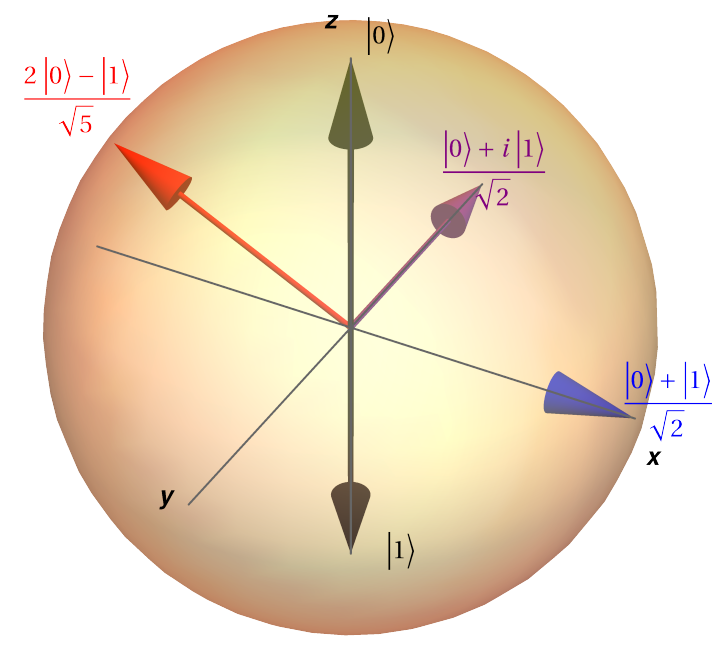
\includegraphics[width=5cm]
{img-congreso/bloch.png}
\end{minipage}
$\stackrel{\E_{z}\otimes\1 \vspace{1cm}}{\longmapsto}$
\begin{minipage}{0.4\textwidth}
\centering
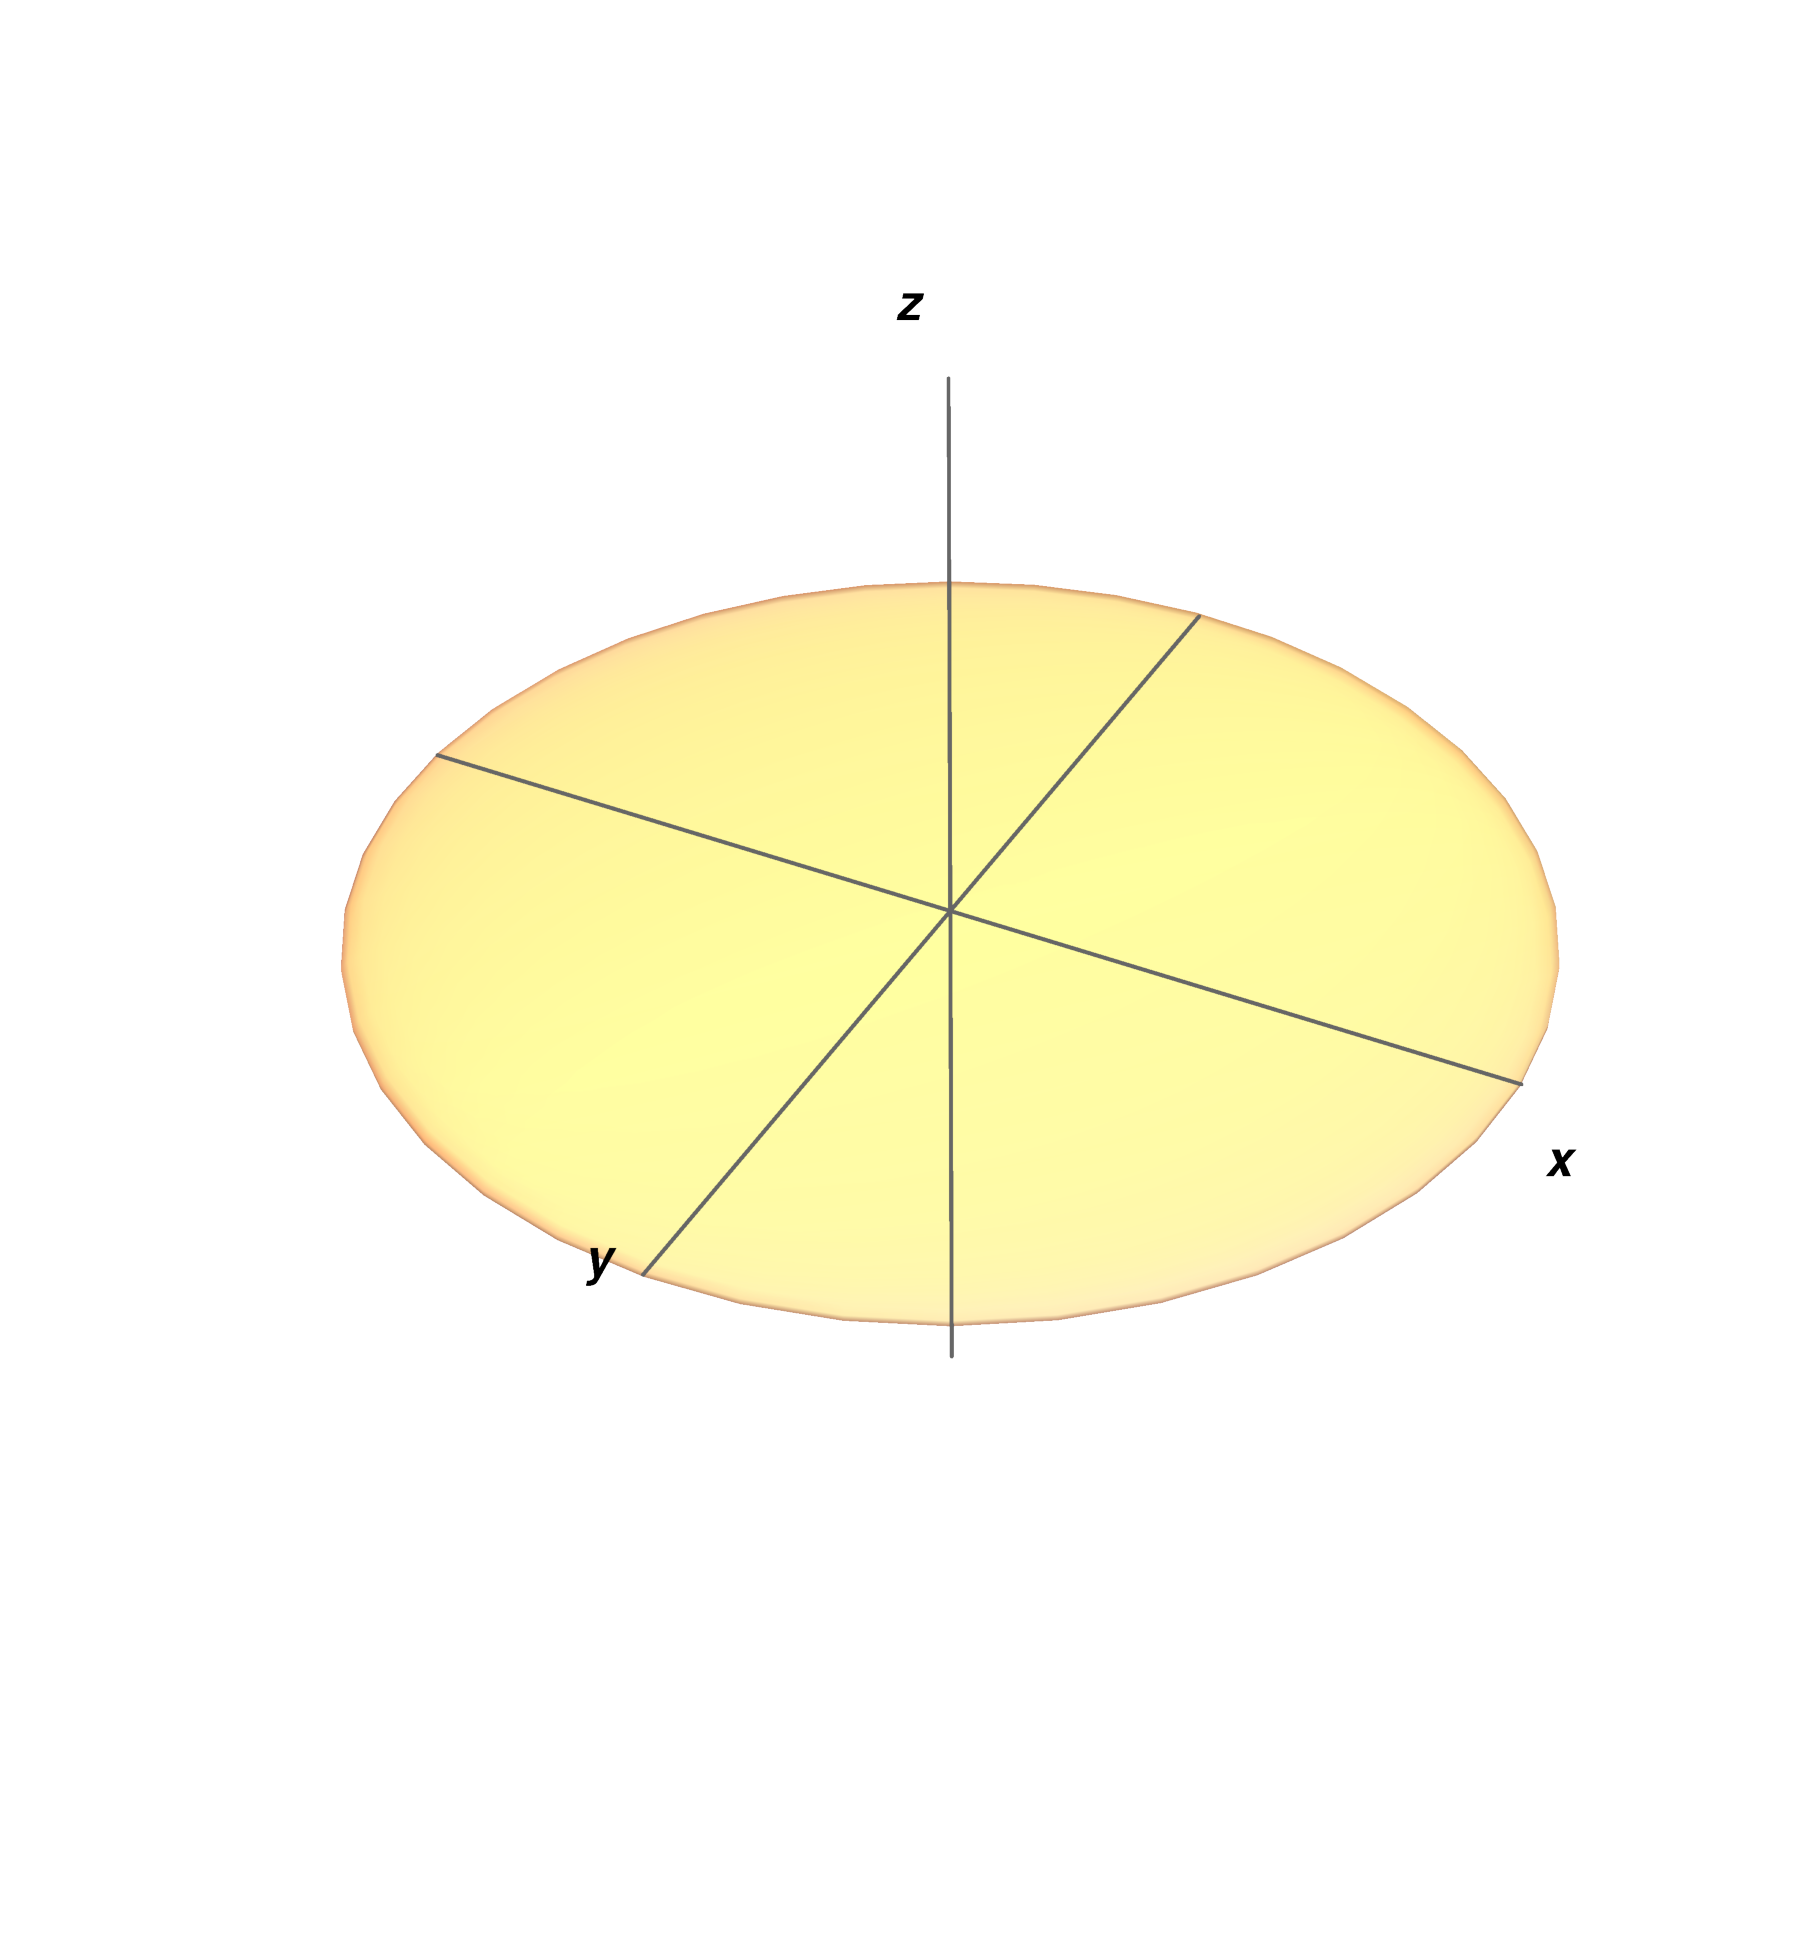
\includegraphics[width=6cm]
{img-congreso/DiskXY}
\end{minipage}
\caption{Deformación de la esfera de Bloch a un disco sobre el plano $XY$.}
\label{fig:qtm-op-motivation}
\end{figure}
Por otro lado, el estado máximente entralazado $\rho^{\phi}$ de 
un sistema de 2 qubits es \cite{bengtsson_zyczkowski_2017}
\begin{align}
\rho^{\phi}&=
\mqty( 
\frac{1}{2} & 0 & 0 & \frac{1}{2} \\
0 & 0 & 0 & 0 \\
0 & 0 & 0 & 0 \\
\frac{1}{2} & 0 & 0 & \frac{1}{2} \\
).
\label{eq:DM-2q-MaxE}
\end{align}
Siguiendo la representación de la matriz de densidad de 1 qubit,
la matriz de densidad de 2 qubits se puede escribir como
\begin{align}
\rho&=\frac{1}{4}\sum _{i,j=0}^{3}r_{ij}\sigma_i\otimes\sigma_j,
\label{eq:DM-2q}
\end{align}
donde $\sigma_0=\1$ y $\vec{r}$ es un vector de 16 entradas que contiene
la información física local de cada qubit y las correlaciones del sistema.
%\janote{por qué se iguala?}
Se igualan \eqref{eq:DM-2q-MaxE} y \eqref{eq:DM-2q} para encontrar
el estado máximamente entrelazado en la representación de \eqref{eq:DM-2q}. 
Se obtiene que $r_{00}=r_{11}=r_{33}=1$, $r_{22}=-1$, y el resto de 
componentes en $\vec{r}$ son iguales a cero. 

Ahora consideremos la operación $\E_z\otimes\1$ que borra
la componente en $z$ del primer qubit y deja invariante 
al segundo qubit. La acción de esta operación es equivalente 
a transformar el vector $\vec{r}$ de $\rho^{\phi}$, en la representación
de \eqref{eq:DM-2q}, como
\begin{align}
\qty(1,0,0,0,0,1,0,0,0,0,-1,0,0,0,0,1)
\longmapsto
\qty(1,0,0,0,0,1,0,0,0,0,-1,0,0,0,0,0).
\end{align}
Por consiguiente, la matriz de densidad $\rho^{\phi}$ se transforma 
ante la operación $\E_z\otimes\1$ como
\begin{align}
\mqty( 
\frac{1}{2} & 0 & 0 & \frac{1}{2} \\
0 & 0 & 0 & 0 \\
0 & 0 & 0 & 0 \\
\frac{1}{2} & 0 & 0 & \frac{1}{2} \\
)
%\E\otimes\1\qty(\rho^{\phi})&=
\stackrel{\E_{z}\otimes\1}{\longmapsto}
\mqty( 
\frac{1}{4} & 0 & 0 & \frac{1}{2} \\
0 & \frac{1}{4} & 0 & 0 \\
0 & 0 & \frac{1}{4} & 0 \\
\frac{1}{2} & 0 & 0 & \frac{1}{4} \\
).
\end{align}
La matriz $\E_z\otimes\1\qty(\rho^{\phi})$ tiene un autovalor igual a $-1/4$.
Por consiguiente, $\E_z\otimes\1\qty(\rho^{\phi})$ no es una matriz 
de densidad. \ccnote{¿qué tiene que ver el autovalor con que no sea matriz de densidad?} Dicho de otro modo, $\E_z\otimes\1\qty(\rho^{\phi})$ 
no describe a algún estado físico de un sistema de 2 qubits.
En resumen, hemos probado que la operación $\E_z$ que deforma la bola 
de Bloch a un disco sobre el plano $XY$, cuando se considera su 
extensión sobre el espacio de 2 qubits $\E_z\otimes\1$ y se aplica al
estado máximamente entrelazado da como resultado un estado no físico. 
En consecuencia, $\E_z$ no representa ninguna evolución física. Este 
resultado deja en evidencia que una operación cuántica debe ser 
un mapeo afín de estados cuánticos, de un sistema que se compone del
sistema principal y otro secundario, sin importar la dimensión del
espacio secundario.

%\janote{- Definición de CP del Geometry of Quantum States.}

Revisemos ahora la definición formal de completa positividad.
Una operación $\E$ se dice que es completamente positiva (CP)
si y sólo si, para cualquier extensión dimensional arbitraria $K$ 
del espacio de Hilbert, tal que 
$\hi_N \rightarrow \hi_N \otimes \hi_K$,
el operador $\E\otimes\1_K$ es positivo semidefinido 
\cite{bengtsson_zyczkowski_2017}. Esta es la última condición 
necesaria de imponer sobre las operaciones cuánticas para 
que sean transformaciones de estados físicos. 

%\janote{- Concluir con que las operaciones que estudiamos deben ser CPTP.}

En conclusión, una operación cuántica es una mapeo afín de 
operadores de densidad que es completamente positivo. 
En la literatura se suele hacer una diferencia entre operaciones cuánticas
y canales cuánticos \cite{weedbrook2012gaussian}, el término operaciones 
cuánticas se utiliza para operaciones que, en general, disminuyen la traza 
del operador de densidad, y canales cuánticos es exclusivo para operaciones 
que preservan la traza del operador de densitad (operaciones CPTP). En 
este proyecto estamos interesados en estudiar las operaciones CPTP. 
En las siguientes dos secciones vamos a presentar dos representaciones
de las operaciones CPTP. 



\section{Superoperadores}
\janote{Propongo agregar esta sección por la línea que quiero seguir 
durante todo el capítulo. Además que si menciono la representación en 
suma de operadores, por qué no la de superoperadores?  es la que he 
usado para la parte numérica}

Una forma de representar a las operaciones cuánticas es la forma de 
superoperadores. Un superoperador es una transformación lineal
que actúa sobre el espacio vectorial de los operadores lineales 
\cite{preskill1998lecture}. Iniciaremos esta sección discutiendo algunas
transformaciones algebraicas sobre matrices e introduciremos 
una notación de cuatro índices para trabajar en un espacio de Hilbert 
compuesto por dos subsistemas. Luego, vamos a presentar 
las condiciones que debe satisfacer un superoperador para ser un 
canal cuántico. Por último vamos a presentar dos ejemplos de operaciones
lineales que actúan sobre el operador de densidad de 1 qubit. En el primer 
ejemplo vamos a retomar la operación discutida en la sección anterior y, 
utilizando su representación de superoperador, vamos a mostrar que no es CP. 
En el segundo discutiremos una operación CP sobre la esfera de Bloch. 

%- Empezar hablando del reshape a $\rho$ (pasarlo de matriz a vector columna)
En la forma de superoperadores de las operaciones cuánticas se 
considera que el superoperador actúa sobre
un vector columna, por lo cual es necesario estudiar alguna transformación
lineal que reordene una matriz en un vector columna, y viceversa.
Consideremos una matriz rectangular $A$ de dimensión $M\times N$.
La matriz puede reordenarse colocando sus elementos de matriz en 
orden lexicográfico \ccnote{qué elegancia la de francia} en un vector $\vec{a}$ con $MN$ elementos, es decir
\begin{align}
a_k=A_{ij}, 
\label{eq:matrix-to-vector}
\end{align}
donde $k=\qty(i-1)N+j$, con $i=,1,\ldots,M$ y $j=1,\ldots,N$. De
esta manera, es posible reordenar a la matriz de densidad como un 
vector columna. Ante esta transformación los elementos de matriz no se 
modifican, por lo cual la información física contenida en una matriz 
de densidad tampoco se altera.

Para determinar si una operación lineal, en su forma de superoperador, es CP 
se evalúa la positividad semidefinida del superoperador
reordenado según el procedimiento de \textit{reshuffle}.
La transformación de \textit{reshuffle} $R$ de una matriz cuadrada $B$ 
consiste en reordenar cada fila de $B$, con $MN$ elementos, 
en submatrices de dimensión $M\times N$ y colocarlas en 
orden lexicográfico bloque por bloque. Veamos un ejemplo del 
\textit{reshuffle} de una matriz $B$ de $4\times 4$, en la que 
cada fila se reordena en una submatriz de $2\times 2$
\begin{align}
B=
\mqty(
B_{00}&B_{01}&B_{02}&B_{03}\\
B_{10}&B_{11}&B_{12}&B_{13}\\
B_{20}&B_{21}&B_{22}&B_{23}\\
B_{30}&B_{31}&B_{32}&B_{33})
\stackrel{R}{\longrightarrow}
\mqty(
B_{00}&B_{01}&B_{10}&B_{11}\\
B_{02}&B_{03}&B_{12}&B_{13}\\
B_{20}&B_{21}&B_{30}&B_{31}\\
B_{22}&B_{23}&B_{32}&B_{33})
=B^R.
\label{eq:reshuffle}
\end{align}
Más adelante veremos que la matriz del superoperador 
reordenada según el \textit{reshuffle} se define como la matriz de Choi
de la operación lineal.

Para establecer las condiciones que una operación en su
representación de superoperador debe cumplir para ser un mapeo afín de
operadores de densidad es útil introducir la siguiente notación de cuatro índices. 
Supongamos que $U$ es un operador que actúa sobre un espacio de Hilbert 
compuesto de la forma $\hi=\hi_M\otimes\hi_N$.
Sea $\ket{i}$ una base ortonormal de $\hi_M$ y $\ket{\mu}$ una base
ortonormal de $\hi_N$. Nótese el uso de letras latinas para los índices del
primer subsistema y letras griegas para los índices del segundo.
El producto tensorial $\ket{i}\otimes\ket{\mu}$
es una base del espacio compuesto $\hi$. Por lo tanto, un 
elemento de matriz de $U$, utilizando cuatro índices, es
\begin{align}
U_\ind{m\mu}{n\nu}=\matrixel{i\otimes \mu}{U}{j\otimes \nu}.
\label{eq:4indices}
\end{align}
\janote{Hablar de los mapeos que actúan sobre $\rho$ como un vector columna}

Hasta ahora lo que hemos expuesto nos permite reordenar a una matriz
de densidad $\rho$ de dimensión $N\times N$ en un vector con $N^2$ 
elementos. Por consiguiente, la representación matricial de un 
superoperador $\E$ que actúa sobre un operador de densidad vectorizado $\vec{\rho}$ 
debe ser de dimensión $N^2\times N^2$. Los elementos de matriz de
$\E$ pueden etiquetarse utilizando cuatro índices como en \eqref{eq:4indices}
haciendo cualquier partición en dos del sistema total.

Una operación $\E$ que sea candidato a canal cuántico debe transformar 
operadores de densidad en operadores de densidad. Esto quiere decir que
la imagen $\rho'$ del operador de densidad debe ser Hermítica, 
de traza unitaria y positiva semidefinida. 
Cada una de estas condiciones sobre $\rho'$ impone una condición 
sobre el superoperador $\E$:
\begin{align}
\txt{(i)}&& \rho'=\qty(\rho')^{\dagger}&&\Leftrightarrow
    && \E_\ind{m\mu}{n\nu}=\E_\ind{\mu m}{\nu n}^*,&&
    \label{eq:H-condition}\\
\txt{(ii)}&&\Tr(\rho')=1
    &&\Leftrightarrow&&  \E_\ind{mm}{n\nu}=\delta_{n\nu},\\     
\txt{(iii)}&&\rho'\geq1
    &&\Leftrightarrow&&  \E_\ind{m\mu}{n\nu}\rho_{n\nu}\geq0.
    \label{eq:positivity-condition}
\end{align}


\janote{
- Hablar de la matriz de Choi y enunciar el teorema de Choi: si la matriz
 de Choi es positiva semidefinida entonces la operación cuántica es CP
}

Según lo que discutimos en la sección anterior estas condiciones
no son suficientes para que $\E$ sea un canal cuántico; adicionalmente 
$\E$ debe ser CP. Para evaluar la completa positividad del superoperador $\E$ 
vamos a definir la matriz de Choi $D_{\E}$ como 
\cite{bengtsson_zyczkowski_2017}
\begin{align}
D_{\E}=\E^{R}.
\end{align}
La matriz de Choi de $\E$ es la matriz que resulta del \textit{reshuffle}
de $\E$. Con la matriz de Choi $D_{\E}$ definida vamos a enunciar 
el teorema de Choi \cite{bengtsson_zyczkowski_2017} que
establece si $\E$ es CP evaluando la positividad semidefinida de $D_{\E}$.
\begin{teorema}
Una transformación lineal $\E$ es completamente positiva si y sólo si 
su matriz de Choi asociada $D_{\E}$ es positiva semidefinida.
\end{teorema}
Este teorema completa las herramientas para establecer el procedimiento 
para evaluar si un superoperador $\E$ es un canal cuántico. 
Dado que $\E$ cumple con las condiciones establecidas en
\eqref{eq:H-condition} a \eqref{eq:positivity-condition}, la positividad
de la matriz de Choi $D_{\E}$ determina si la operación es un canal cuántico.

\janote{
- Concluir con un ejemplo de un canal nuestro sobre 1 qubit
}

Retomemos el ejemplo de la operación $\E_z$ sobre 1 qubit de la sección anterior
que se ilustra en la \Fref{fig:qtm-op-motivation}. La ecuación \eqref{eq:E(rho)}
de la transformación del operador de densidad por un canal cuántico, 
considerando al superoperador $\E_z$ y a la matriz de densidad 
$\rho$ de 1 qubit, en \eqref{eq:DM-1q}, como un vector según la ecuación 
\eqref{eq:matrix-to-vector}, es 
\begin{align}
\mqty(
\frac{1}{2} & 0 & 0 & \frac{1}{2} \\
0 & 1 & 0 & 0 \\
0 & 0 & 1 & 0 \\
\frac{1}{2} & 0 & 0 & \frac{1}{2} \\
)
\frac{1}{2}
\mqty(
1+r_z\\r_x-ir_y\\r_x+ir_y\\1-r_z
)
=
\frac{1}{2}
\mqty(
1\\r_x-ir_y\\r_x+ir_y\\1
)
\end{align}
Se calcula la matriz de Choi $\E_z^{R}$, siguiendo la ecuación
\eqref{eq:DM-1q},
\begin{align}
\E_z^R=
\mqty(
\frac{1}{2} & 0 & 0 & 1 \\
0 & \frac{1}{2} & 0 & 0 \\
0 & 0 & \frac{1}{2} & 0 \\
1 & 0 & 0 & \frac{1}{2} 
).
\end{align}
La matriz $\E_z^R$ tiene un autovalor $-1/2$, por ello $\E_z$ no es CP y,
por consiguiente, no es un canal cuántico. Nótese que hemos llegado a la misma 
conclusión de la sección anterior sobre la CP, pero utilizando la representación 
de superoperador de $\E_z$.

\janote{Otro ejemplo, pero ahora sí de un canal}

Para concluir la sección será útil desarrollar un ejemplo más 
de una operación CP sobre un sistema de 1 qubit. Este 
ejemplo servirá para proporcionar más familiaridad con la representación de 
los superoperadores y para hacer la conexión con 
la forma de Kraus de las operaciones CP en la siguiente sección.

Consideremos la operación $\E_{xz}$ que colapsa la esfera de Bloch de 
un sistema de 1 qubit al eje $y$, como se muestra en la \Fref{fig:QC-ex2}.
\begin{figure}[H]
    \centering
    \begin{minipage}{.4\textwidth}
        \centering
        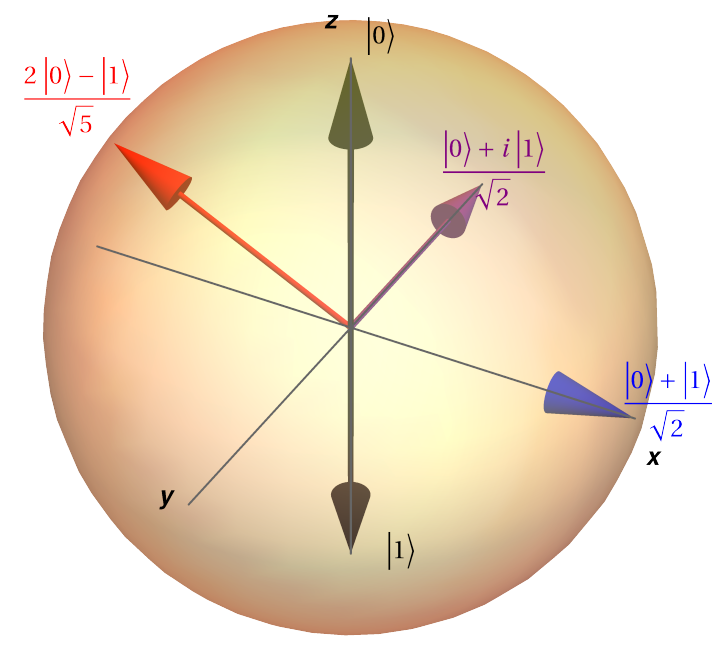
\includegraphics[width=5cm]
        {img-congreso/bloch.png}
    \end{minipage}
    $\stackrel{\E_{xz}\otimes\1 \vspace{1cm}}{\longmapsto}$
    \begin{minipage}{0.4\textwidth}
        \centering
        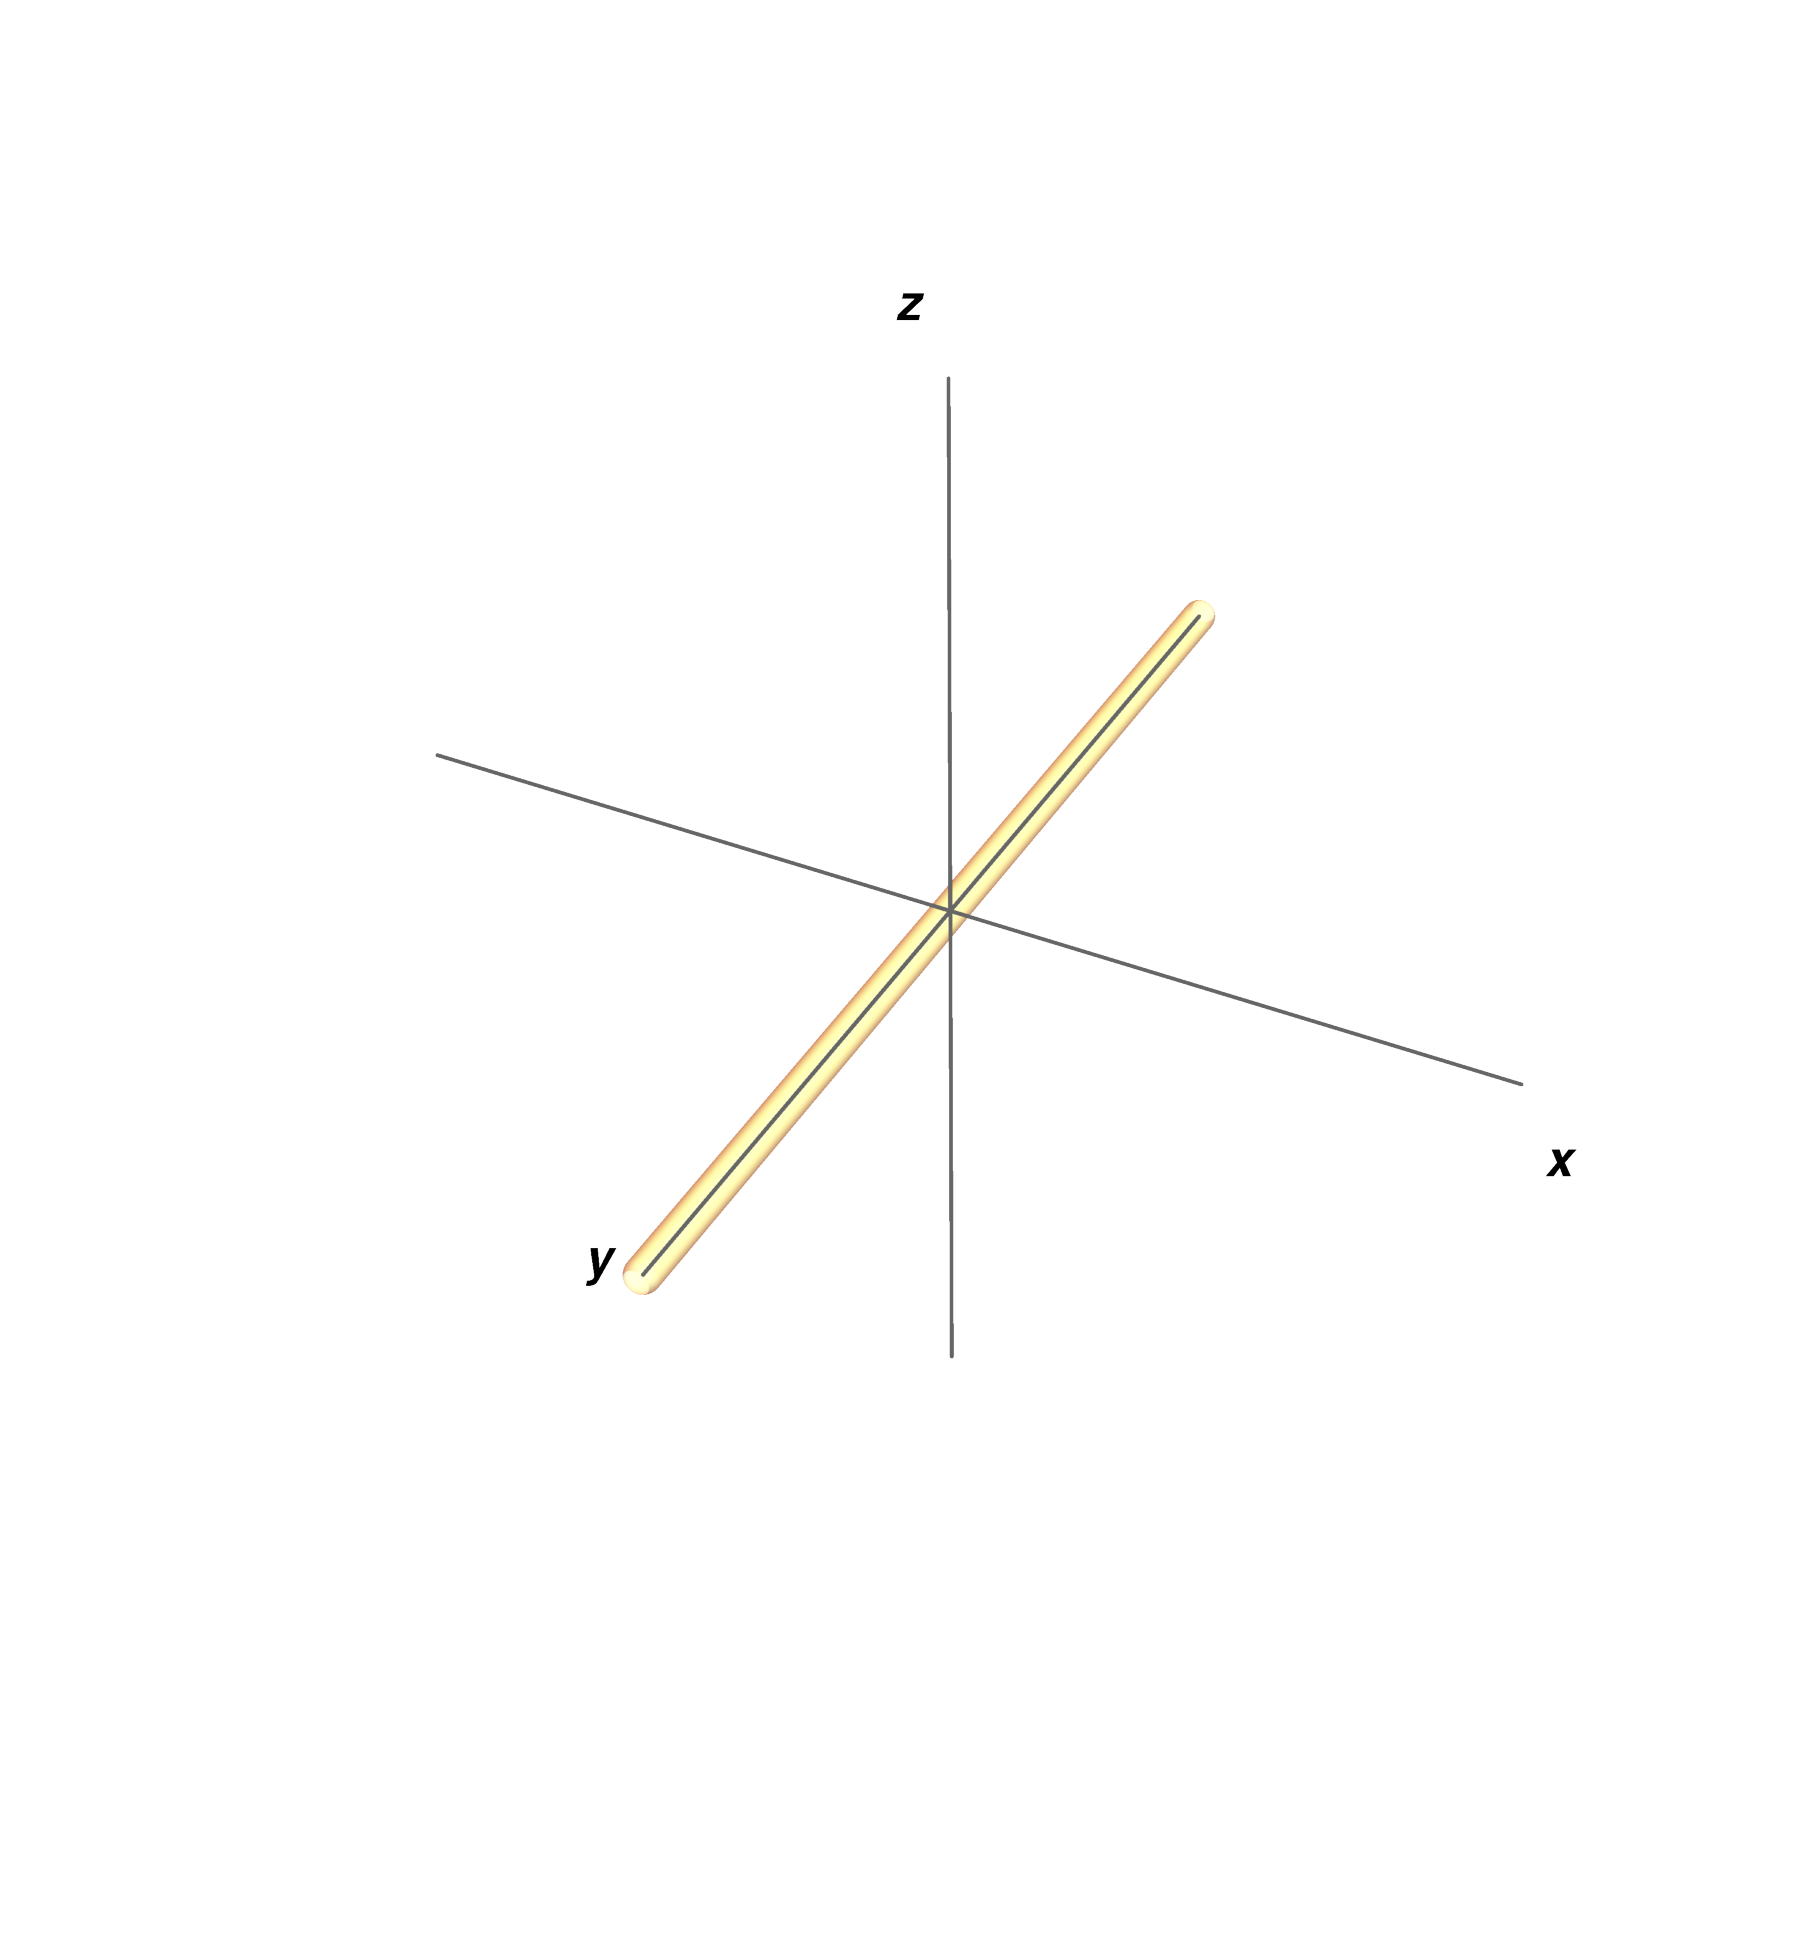
\includegraphics[width=6cm]
        {img-congreso/lineY}
    \end{minipage}
    \caption{Deformación de la esfera de Bloch a un disco sobre el plano $XY$.}
    \label{fig:QC-ex2}
\end{figure}
La transformación de los estados de 1 qubit en la esfera de Bloch 
según la operación $\E_{xz}$ está descrita por la siguiente ecuación
\begin{align}
\mqty(
\begin{array}{cccc}
\frac{1}{2} & 0 & 0 & \frac{1}{2} \\
0 & \frac{1}{2} & -\frac{1}{2} & 0 \\
0 & -\frac{1}{2} & \frac{1}{2} & 0 \\
\frac{1}{2} & 0 & 0 & \frac{1}{2} \\
\end{array}
)
\frac{1}{2}
\mqty(
1+r_z\\r_x-ir_y\\r_x+ir_y\\1-r_z
)
=
\frac{1}{2}
\mqty(
1\\-ir_y\\ir_y\\1
),
\label{eq:QC-ex2-SR}
\end{align}
donde la matriz es el superoperador $\E_{xz}$. 
Para comprobar si la matriz en \eqref{eq:QC-ex2-SR} es CP debemos 
determinar $\E_{xz}^R$ y verificar si es positiva semidefinida. Notemos que $\E_{xz}^R=\E_{xz}$, por lo tanto, 
$\E_{xz}$ es CP y, porque además satisface las condiciones
\eqref{eq:H-condition} a \eqref{eq:positivity-condition}, es un canal cuántico.
´
En resumen, la representación en superoperador de una operación cuántica
se trata de reordenar la matriz de densidad $\rho$ como 
un vector columna y considerar la transformación que actúa sobre el nuevo
vector $\vec{\rho}$. Si un operación $\E$ satisface las condiciones
\eqref{eq:H-condition} a \eqref{eq:positivity-condition}, entonces
es un mapeo afín de matrices de densidad.
Por otro lado, el procedimiento de \textit{reshuffle} 
nos proporciona un procedimiento para calcular la matriz de Choi de una 
operación $\E$. Seguidamente, el teorema de Choi establece que si 
la matriz de Choi es positiva semidefinida, entonces $\E$ es CP. 
De esta manera, hemos establecido las herramientas para evaluar 
si una operación en su forma de superoperador es un canal cuántico.
En la siguiente sección discutiremos otra forma de representar a las operaciones
cuánticas.

\section{Forma de Kraus}
\janote{
- Enunciar la representación en operadores de suma partiendo de un 
estado que se acopla con algún entorno
y llegar a las condiciones para ser CPTP y empezar a conectarlo
con la sección anterior.} \cpnote{No sabes si hay alguna motivacion que no sea
con el entorno? Realmente no lo usamos y se me hace meter una complicación adicional}
\janote{Entonces voy a omitir la motivación con el entorno.}

\janote{Introducción:\\ \indent}
Las operaciones cuánticas tienen otra representación distinta a la de 
los superoperadores que se conoce como la forma de Kraus. La diferencia
principal entre ambas representaciones es que la forma de los superoperadores
considera operadores que actúan sobre el espacio de los operadores lineales, y
la forma de Kraus considera operadores que actúan sobre el espacio de 
Hilbert del sistema. Vamos a iniciar retomando el segundo ejemplo de la sección 
anterior, en el cual estudiamos la operación $\E_{xz}$ cuya acción sobre la esfera
de Bloch se muestra en la \Fref{fig:QC-ex2}.
Vamos a mostrar cómo encontrar la forma de Kraus de $\E_{xz}$ 
a partir de la forma de superoperador del canal cuántico.
Después, vamos a concluir presentando las condiciones 
de la forma de Kraus de una operación para que sea un canal cuántico.

\janote{
- Invocar el ejemplo del canal de la sección anterior, pero en su 
representación de operadores de suma. Aquí quiero hacer la conexión 
entre esta y la sección anterior mostrando que los operadores 
de Kraus son los autovectores de la matriz de Choi.}

Recordemos que el canal cuántico $\E_{xz}$ es una operación
que colapsa la esfera de Bloch a una línea sobre el eje $y$, 
como se muestra en la \Fref{fig:QC-ex2}. 
La matriz en la ecuación \eqref{eq:QC-ex2-SR} representa al canal cuántico
en su forma de superoperador. Notemos que su matriz de Choi $\E_{xz}^R$
asociada es ella misma $\qty(\E_{xz}^R=\E_{xz})$. 
Consideremos los autovectores $\ket{E_{1,2,3,4}}$ de $\E_{xz}^R$:
\begin{align}
\ket{E_{1,2,3,4}}=
\mqty(\frac{1}{2},0,0,\frac{1}{2})^T,
\mqty(0,-\frac{1}{2},\frac{1}{2},0)^T,
\mqty(-\frac{1}{2},0,0,\frac{1}{2})^T,
\mqty(0,\frac{1}{2},\frac{1}{2},0)^T;
\end{align}
cuyos autovalores son $\lambda_{1,2,3,4}=1/2,1/2,0,0$, respectivamente.
Si tomamos a $\ket{E_1}$ y $\ket{E_2}$, los únicos autovectores
con autovalores distintos de cero, y los reordenamos en 
las matrices $E_1$ y $E_2$, de dimensión $2\times2$, siguiendo 
el procedimiento inverso de vectorización en \eqref{eq:matrix-to-vector} 
se obtienen
\begin{align}
E_0&=
\frac{1}{\sqrt{2}}
\mqty(
1 & 0\\
0 & 1
),
&
E_1&=
\frac{1}{\sqrt{2}}
\mqty(
0 & -1\\
1 & 0
).
\end{align}
Si ahora consideramos la operación
\begin{align}
\rho'=\sum_{i=0}^1E_i\rho E_i^{\dagger},
\label{eq:Kraus}
\end{align}
donde $\rho$ es la matriz de densidad de 1 qubit en \eqref{eq:DM-1q}, 
entonces
\begin{align}
\rho'=&
\frac{1}{2}
\mqty(
1 & 0\\
0 & 1
)
\mqty(
\frac{1+r_z}{2}& \frac{r_x-ir_y}{2}\\
\frac{r_x+ir_y}{2} & \frac{1-r_z}{2}
)
\mqty(
1 & 0\\
0 & 1
)
+
\frac{1}{2}
\mqty(
0 & -1\\
1 & 0
)
\mqty(
\frac{1+r_z}{2}& \frac{r_x-ir_y}{2}\\
\frac{r_x+ir_y}{2} & \frac{1-r_z}{2}
)
\mqty(
0 & 1\\
-1 & 0
)&
\nonumber\\
\rho'=&
\frac{1}{2}
\mqty(
1 & -ir_y\\
ir_y & 1
).
\label{eq:QC-ex2-KR}
\end{align}
Hemos obtenido el mismo resultado, pero reordenado como matriz,
de la ecuación \eqref{eq:QC-ex2-SR}. No obstante, las operaciones que 
realizamos sobre la matriz de densidad fueron
con operadores que también actúan sobre el espacio de Hilbert de 1 qubit. 
La ecuación \eqref{eq:Kraus} se conoce 
como la forma de \textit{Kraus} de los mapeos completamente positivos
\cite{bengtsson_zyczkowski_2017}.
Los autovectores de la matriz de Choi de una operación cuántica $\E$ 
reordenados como matrices se
conocen como los operadores de Kraus $E_i$ de $\E$.
Los operadores $E_i$ linealmente independientes 
pueden ser hasta $N^2$ \cite{nielsen_chuang_2011}, igual a la dimensión 
del espacio de los operadores lineales que actúan sobre un espacio de
Hilbert de dimensión $N$. 
Una operación cuántica $\E$ preserva la traza de la matriz de densidad 
si y sólo sus operadores de Kraus $E_i$ satisfacen la condición
\cite{bengtsson_zyczkowski_2017}
\begin{align}
\sum_iE_i^{\dagger}E_i=\1.
\label{eq:kraus-tp-cond}
\end{align}
\janote{
- Comparar la representacion de suma de operadores y superoperadores\\ \indent}
En resumen, las ecuaciones \eqref{eq:Kraus} y \eqref{eq:kraus-tp-cond}
caracterizan la forma de Kraus de un canal cuántico. 
Con esto hemos mostrado dos formas distintas de representar a un 
canal cuántico: la forma de superoperador, una matriz cuadrada
de dimensión $N^2$, que actúa sobre una matriz de densidad vectorizada 
con $N^2$ entradas; y la forma de Kraus, matrices de dimensión $N$
que actúan sobre una matriz de densidad de dimensión $N$. La matriz de 
Choi del canal cuántico proporciona una manera de conectar ambas 
representaciones. Por un lado, si $D_{\E}$ es la matriz de Choi de un canal 
cuántico $\E$, entonces $D_{\E}^R$ es la representación matricial
del canal en su forma de superoperador.
Por otro lado, los autovectores de $D_{\E}$
multiplicados por la raíz cuadrada de sus autovalores asociados 
son los operadores de Kraus del canal cuántico. 

\janote{No me parece necesario entrar en detalle con la forma de Kraus.
Quizás las demostraciones y más detalle se pueden guardar para la tesis.
Espero haber logrado dar una buena motivación de la CP y haber conectado
bien la forma de Kraus con la de superoperadores con los ejemplos.}
\section{Canales cuánticos de 1 qubit}
\janote{
- Hablar de que se gana intuición pensando en la acción de un canal de 1
qubit como la manera en que deforma la esfera de Bloch}


\janote{
- Ejemplos: phase-flip channel, depolarizing y amplitude damping\\ \indent}
Algunos ejemplos de canales cuánticos de un sistema de 1 qubit 
pueden proporcionar intuición 
para completar el esquema de los canales cuánticos. 
Como se presentó en los ejemplos que abordamos en las 
secciones anteriores, los sistemas de 1 qubit ofrecen la
herramienta geométrica de la esfera de Bloch para asociar cada 
punto de ella con un estado del sistema. De esa manera, 
se puede visualizar la acción de un canal cuántico como la 
deformación de la esfera de Bloch bajo la acción del canal.
En esta sección vamos a estudiar la acción de tres canales 
cuánticos representativos sobre un sistema de 1 qubit. Presentaremos
tanto la forma de superoperador como la forma de Kraus de 
cada uno de los canales cuánticos.

El primer ejemplo a presentar es el canal \textit{bit-phase flip} $\E_{BPF}$. 
Con probabilidad $1-p$, el canal $\E_{BPF}$ intercambia 
los estados $\ket{0}$ y $\ket{1}$, 
autoestados de $\sigma_z$, e intercambia la fase total
del estado $\ket{\psi}$ del qubit. 
Recordemos que la matriz de densidad en \eqref{eq:DM-1q} 
las coordenadas $r_i$ en la esfera de Bloch del punto asociado al estado
del sistema. La acción de $\E_{BPF}$ es 
equivalente a la siguiente transformación del vector de Bloch $\vec{r}$
\begin{align}
\qty(r_x,r_y,r_z)\rightarrow&\Big(\qty(1-2p)r_x,r_y,\qty(1-2p)r_z\Big).
\label{eq:bit-phase-flip-Bloch-trans}
\end{align}
Geométricamente, el vector de Bloch es proyectado por el canal 
al eje $y$ y las componentes en $x$ y $z$ son perdidas, como 
se muestra en la \Fref{fig:bit-phase-flip}.
Notemos que el ejemplo que discutimos en la sección 2.2 del 
canal cuántico que colapsa la esfera de Bloch al eje $y$ es un caso
particular de $\E_{BPF}$ cuando $p=0.5$.
\begin{figure}[H]
\centering
\begin{minipage}{.4\textwidth}
    \centering
    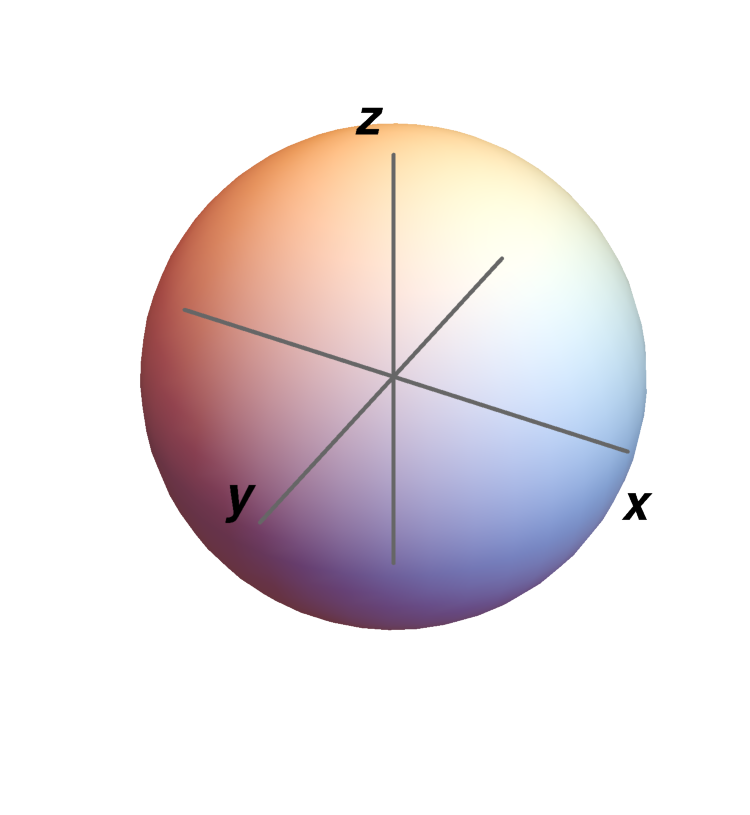
\includegraphics[width=6cm]{images/bloch-ball}
\end{minipage}
$\longmapsto$
\begin{minipage}{0.4\textwidth}
    \centering
    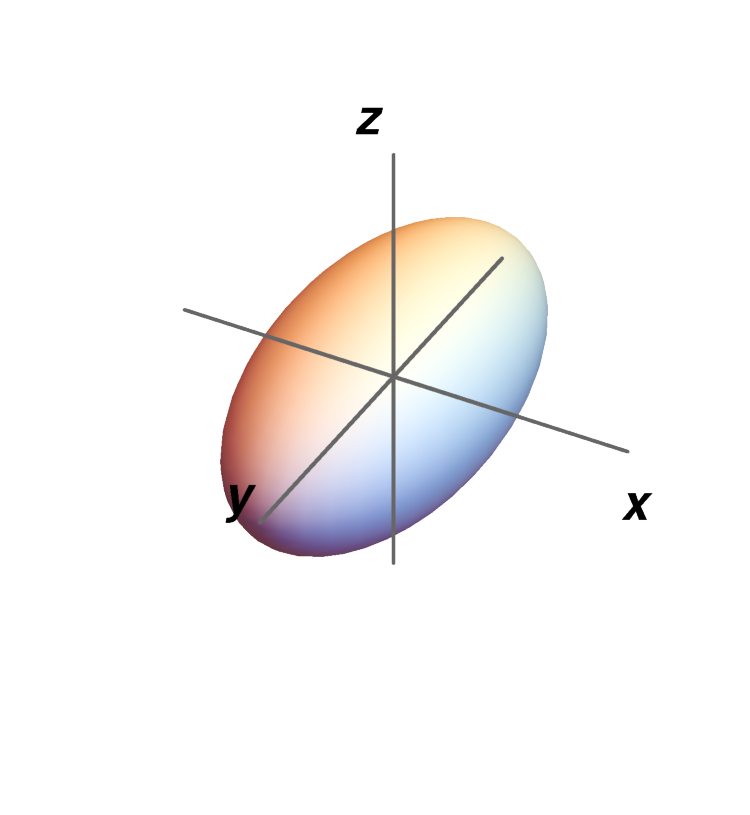
\includegraphics[width=6cm]{images/bit-phase-flip}
\end{minipage}
\caption{Efecto del canal \textit{bit-phase flip} sobre la esfera de Bloch, 
para $p=0.3$.}
\label{fig:bit-phase-flip}
\end{figure}
La expresión en \eqref{eq:bit-phase-flip-Bloch-trans} nos 
permite calcular la matriz de densidad $\rho'$ que resulta
bajo la acción del canal \textit{bit-phase flip}. Por lo tanto, 
vectorizando $\rho$, $\rho'$ y aplicando métodos elementales de
álgebra lineal se encuentra que la ecuación de transformación de
la matriz de densidad de 1 qubit en la forma de superoperador 
de $\E_{BPF}$ es
\begin{align}
\frac{1}{2}
\mqty(
1-p & 0 & 0 & p \\
0 & 1-p & -p & 0 \\
0 & -p & 1-p & 0 \\
p & 0 & 0 & 1-p \\
)
\frac{1}{2}
\mqty(
1+r_z\\r_x-ir_y\\r_x+ir_y\\1-r_z
)
=
\frac{1}{2}
\mqty(
1+\qty(1-p)z\\
\qty(1-p)x-i y\\
\qty(1-p)x+i y\\
1-\qty(1-p)z
).
\label{eq:bpf-supero}
\end{align}
Para encontrar los operadores de Kraus se determinan los autovectores
de la matriz de Choi $D_{\E_{BPF}}$ del canal \textit{bit-phase flip}. 
Para encontrar la matriz de Choi se aplica la transformación 
de \textit{reshuffle} a la matriz en la ecuación \eqref{eq:bpf-supero}.
Los autovectores de $D_{\E_{BPF}}$, reordenados como matrices y
cada uno multiplicado por la raíz cuadrada de su autovalor respectivo, son
\begin{align}
E_0&=
\sqrt{p}
\mqty(
1 & 0\\
0 & 1
)&
E_1&=
\sqrt{1-p}
\mqty(
0 & -1\\
1 & 0
).
\label{eq:bpf-kraus}
\end{align}
Así hemos encontrado la forma de superoperador y de Kraus del canal
cuántico \textit{bit-phase flip} $\E_{BPF}$. Se puede evaluar directamente que 
tanto la matriz en \eqref{eq:bpf-supero} como los operadores $E_i$
en \eqref{eq:bpf-kraus} cumplen con las condiciones respectivas
para ser canales cuánticos.

Ahora estudiaremos el canal depolarizante $\E_{Dep}$, que se muestra
en la \Fref{fig:depolarizing}, cuya acción sobre el 
vector de Bloch con probabilidad $(1-p)$ es 
\begin{align}
\qty(r_x,r_y,r_z)\rightarrow&\Big(\qty(1-p)r_x,\qty(1-p)r_y,\qty(1-p)r_z\Big).
\label{eq:depolarizing-bloch-vec}
\end{align}
Geométricamente, el canal $\E_{Dep}$ atenúa por igual todas las 
componentes del vector de Bloch y tiene como caso límite $(p=1)$
el mapeo de cualquier estado de 1 qubit al estado 
de máxima ignorancia o máximamente mixto $\1/2$
\cite{bengtsson_zyczkowski_2017}, asociado con el origen de coordenadas.
\begin{figure}[H]
    \centering
    \begin{minipage}{.4\textwidth}
        \centering
        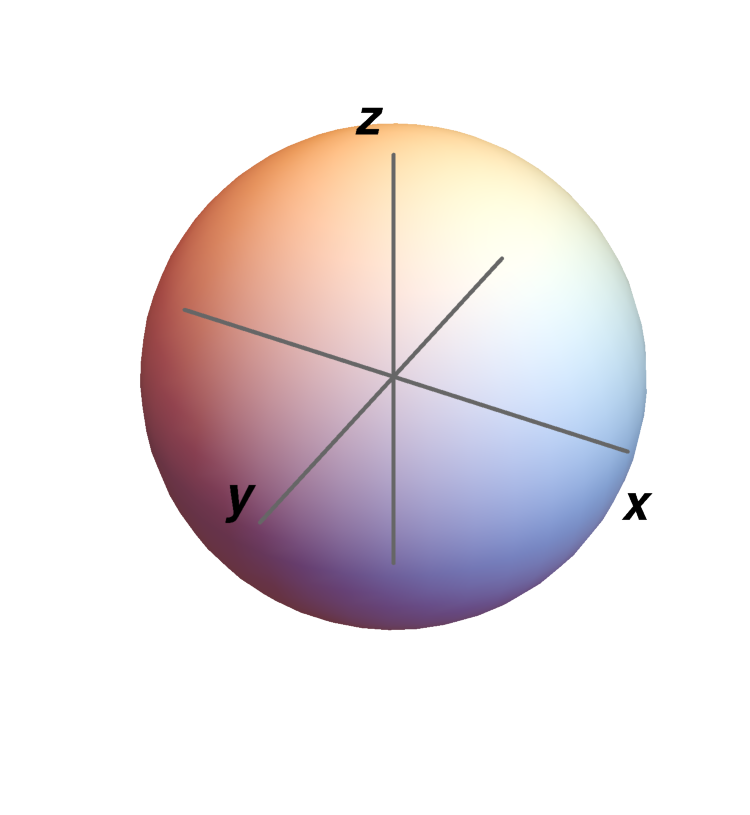
\includegraphics[width=6cm]{images/bloch-ball}
    \end{minipage}
    $\longmapsto$
    \begin{minipage}{0.4\textwidth}
        \centering
        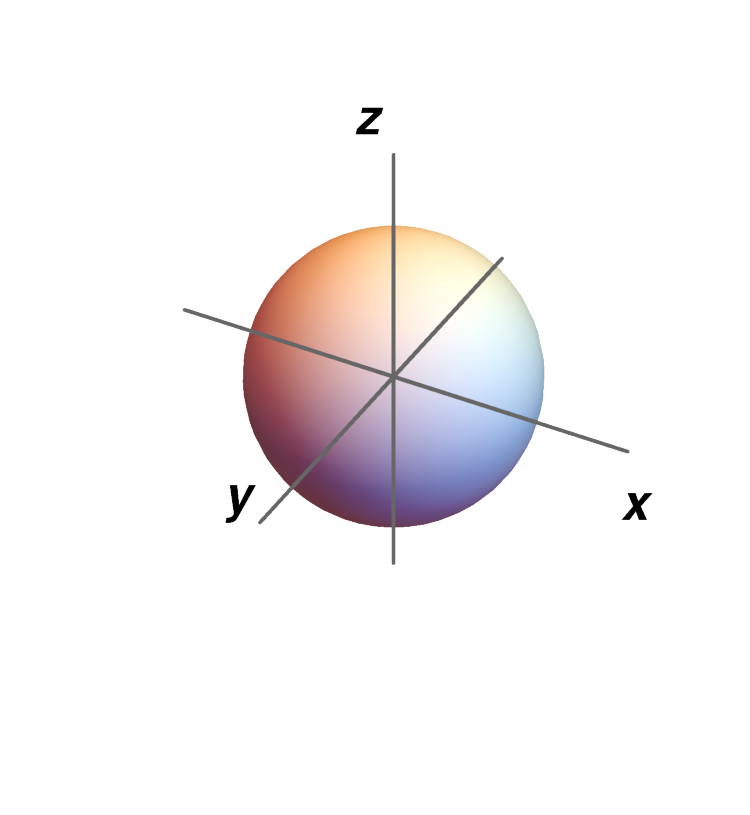
\includegraphics[width=6cm]{images/depolarizing}
    \end{minipage}
    \caption{Efecto del canal depolarizante sobre la esfera de Bloch, 
    para $p=0.4$.}
    \label{fig:depolarizing}
\end{figure}
Repitiendo el procedimiento del ejemplo anterior para calcular 
la ecuación de transformación de la matriz de densidad de
1 qubit bajo la acción de $\E_{Dep}$ en su forma de 
superoperador se encuentra que es
\begin{align}
\frac{1}{2}
\mqty(
1-\frac{p}{2} & 0 & 0 & \frac{p}{2} \\
0 & 1-p & 0 & 0 \\
0 & 0 & 1-p & 0 \\
\frac{p}{2} & 0 & 0 & 1-\frac{p}{2}
)
\frac{1}{2}
\mqty(
1+r_z\\r_x-ir_y\\r_x+ir_y\\1-r_z
)
=
\frac{1}{2}
\mqty(
1+\qty(1-p)z\\
\qty(1-p)\qty(x-i y)\\
\qty(1-p)\qty(x+i y)\\
1-\qty(1-p)z
),
\end{align}
y calculando los autovectores y autovalores de la matriz de Choi de
$\E_{Dep}$ se encuentra que los operadores de Kraus del 
canal depolarizante son
\begin{align}
E_0&=
\sqrt{1-\frac{3p}{4}}
\mqty(
1 & 0\\
0 & 1
),&
E_1&=
\frac{\sqrt{p}}{2}
\mqty(
-1 & 0\\
0 & 1
),\\
E_2&=
\frac{\sqrt{p}}{2}
\mqty(
0 & -1\\
1 & 0
), &
E_3&=
\frac{\sqrt{p}}{2}
\mqty(
0 & 1\\
1 & 0
).
\end{align}
Los dos ejemplos anteriores son canales cuánticos que dejan invariantes 
el estado máximamente mixto. Es decir, $\E(\1/2)=\1/2$. Los canales que
satisfacen esta condición se conocen como canales unitales. El 
último ejemplo a continuación será un canal cuántico que 
no cumple la condición de unitalidad. Geométricamente, esto
se visualiza como un canal cuya acción sobre la esfera de Bloch
la deforma de tal manera que el centro geométrico no se mantiene
en el origen de coordenadas.

\janote{Generalized amplitude damping:\\ \indent}
El último canal cuántico que vamos a estudiar es el canal de
amortiguamiento de fase.
\begin{align}
\mqty(
1 & 0 & 0 & \gamma  \\
0 & \sqrt{1-\gamma } & 0 & 0 \\
0 & 0 & \sqrt{1-\gamma } & 0 \\
0 & 0 & 0 & 1-\gamma
)
\frac{1}{2}
\mqty(
1+r_z\\r_x-ir_y\\r_x+ir_y\\1-r_z
)
=
\frac{1}{2}
\mqty(
1+\gamma+\qty(1-\gamma)z\\
\sqrt{1-\gamma}\qty(x-i y)\\
\sqrt{1-p}\qty(x+i y)\\
1-\gamma-\qty(1-\gamma)z
),
\end{align}
cuyos operadores de Kraus son 
\begin{align}
E_0&=
\sqrt{1-\gamma }
\mqty(
\frac{1}{\sqrt{1-\gamma }} & 0 \\
0 & 1
)&
E_1&=
\sqrt{\gamma }
\mqty(
0 & 1 \\
0 & 0 
)
\end{align}

\begin{figure}[H]
    \centering
    \begin{minipage}{.4\textwidth}
        \centering
        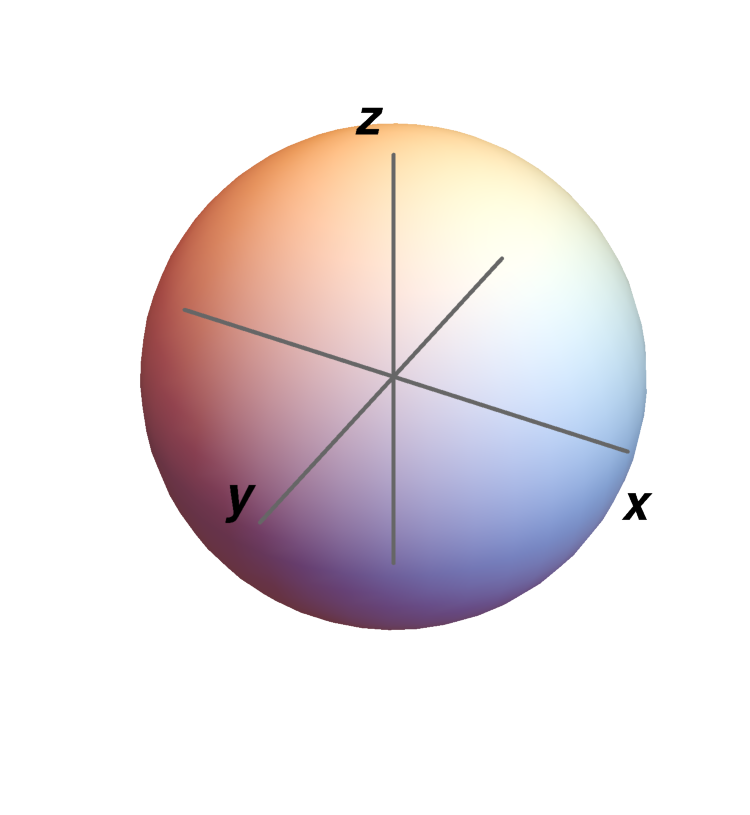
\includegraphics[width=6cm]{images/bloch-ball}
    \end{minipage}
    $\longmapsto$
    \begin{minipage}{0.4\textwidth}
        \centering
        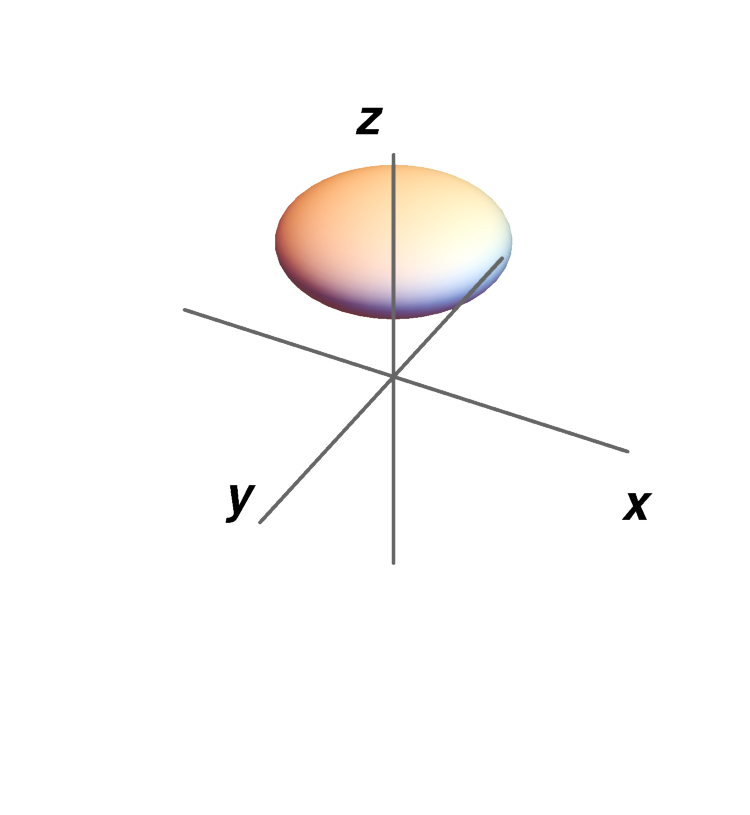
\includegraphics[width=6.2cm]{images/gen-amplitude-damping}
    \end{minipage}
    \caption{Efecto del canal generalizado de amortiguamiento de 
        amplitud sobre la esfera de Bloch, 
        para $p=0.4$.}
    \label{fig:depolarizing}
\end{figure}
\janote{
- De los ejemplos hablar sobre canales unitales? Breve. (es que nuestros
canales son unitales)}

% }}}


\chapter{Mapeos proyectivos}  
% Intro {{{
% \janote{Introducción. Motivar y justificar el estudio de las operaciones
% que borran componentes de la matriz de densidad de un 1 qubit. Discutir
% que entender los canales cuánticos que borran componentes de la 
% matriz de densidad ayudaría a entender mejor la teoría 
% de las operaciones CPTP y, también, la mecánica cuántica porque al fin y al 
% cabo estamos estudiando qué permite y qué no la mecánica 
% cuántica.}
% 
% \cpnote{La justificacion me gustaria ver en pseudocodigo antes de que la afines. 
% Menciona un poco también la relación con los otros mapeos, pero muy por encima, como 
% los de Ruskai}

En la sección 2.1 utilizamos el
ejemplo de una operación lineal 
de 1 qubit que borra una componente del vector de Bloch para motivar
la condición de completa positividad. 
Revisamos que esa operación no es completamente positiva.
Por otro lado, en la sección 2.4.2 revisamos el 
canal depolarizante, un operación cuántica que para $p=1$
borra las 3 componentes del vector de Bloch. En vista de esto, 
inevitablemente salta la pregunta acerca de cuántas (y cuáles) 
componentes del vector de Bloch puede borrar una operación 
de 1 qubit y ser completamente positiva.
Debe hacerse hincapié que las operaciones que borran componentes 
del vector de Bloch son operaciones lineales que 
preservan la traza y la Hermiticidad de la 
matriz de densidad de 1 qubit, por lo que la completa positividad 
es la única condición restante para determinar si la operación 
es un canal cuántico.

%Si bien los canales cuánticos de 1 qubit han sido estudiados y 
%están completamente caracterizados por otros autores
%los canales cuánticos de $n$ qubits aún no~\cite{nielsen_chuang_2011}
%\cite{bengtsson_zyczkowski_2017}\cpnote{Normalmente las citas se ponen al final
%de la frase, menos que no se entienda. Un ejemplo donde toca ponerlas 
%a la mitad de la frase es Hay muchas formas de preparar tacos. La forma
%del norte [1], la del centro [2] y la del sur[3] son cada una diferentes. }. En
%ese sentido \cpnote{Por qué ``en ese sentido?''}, proponemos estudiar las
%operaciones
%que borran componentes del vector de Bloch (generalizado, para el 
%caso de $n$ qubits). Por lo cual, este capítulo se enfoca en  
%estudiar, reproducir y entender las operaciones de 1 qubit 
%que borran componentes del vector de Bloch. \cpnote{Este parrafo siento 
%que no tiene estructura. De que se trata? Hemos hablado de como se estructura 
%típicamente un parrafo? Si no lo hemos hecho, dime y te mando una referencia. Si lo 
%hemos hecho, trata de iterarlo. Se para acá el parrafo anterior de lo que viene 
%explicando la estructura.} En la sección 3.1
%se establece el problema y una solución analítica.
%Por último, en la sección 3.2 se presenta el método numérico que 
%propusimos, así como las herramientas que se utilizaron y 
%los resultados.

\janote{Los siguientes dos párrafos son el reemplazo del párrafo malo 
que estaba antes}
En este capítulo comenzaremos el estudio de las operaciones que 
borran componentes del vector de Bloch con el caso más sencillo de 
1 qubit. Entender por completo el caso de 1 qubits nos proporcionará 
de intuición para empezar a entender las características de las operaciones
de nuestro interés, y también para diseñar una forma de investigar
el caso de sistemas de más qubits. Por otro lado, Bengtsson y Zyczkowski
\cite{bengtsson_zyczkowski_2017} estudiaron 
una caracterización general de los canales cuánticos de 
1 qubit con la cual se puede comparar los resultados de este capítulo 
para hacer una revisión de consistencia \janote{de consistencia está bien 
dicho? Me refiero a hacer un check}. El caso de 1 qubit es importante 
y es el punto de partida para investigar sistemas de más qubits.

La estructura de este capítulo es la siguiente. 
En la sección \ref{sec:caso-1-qubit} vamos a establecer el problema 
de las operaciones que borran componentes del vector de Bloch y 
vamos a revisar un procedimiento analítico para verificar 
la completa positividad de estas operaciones.  
Luego, en la sección \ref{sec:metodo-num},
discutiremos el diseño del método numérico, los resultados y 
una comparación de ellos con la caracterización de los canales 
cuánticos de 1 qubit de Bengtsson y Zyczkowski 
\cite{bengtsson_zyczkowski_2017}.

% }}}
\section{El caso de 1 qubit} \label{sec:caso-1-qubit} % {{{
% \janote{Introducción sobre los canales cuánticos de 1 qubit. Recordar 
% la forma de la matriz de densidad escrita en la representación 
% de Pauli y su asociación con la esfera de Bloch.}

% \janote{Establecer el problema que nos interesa para 1 qubit:
% mapeos que borran y dejan invariantes todas las combinaciones 
% posibles de las componentes del vector de Bloch. 
% Discutir que la componente $r_0$ la dejamos intacta para 
% preservar la traza. Hablar de la representación geométrica 
% de las operaciones que estudiamos.}
% 
% \janote{Presentar la forma analítica de calcular la representación
% en forma de superoperador de alguno de los 8 mapeos posibles. 
% A diferencia de lo que ya se hizo en el capítulo anterior, voy a presentar
% el cálculo a partir de la forma diagonal del mapeo (también para ir 
% dando las herramientas para el algoritmo numérico)}
% 
% \janote{Concluir presentando las 8 operaciones de 1 qubit que nos intersan.}
% \cpnote{Me parece bien, pero porfa no te extiendas de más en este capitulo}

Los canales cuánticos de 1 qubit son especialmente interesantes porque 
son fáciles de visualizar en la esfera de Bloch, como se presentó
en la sección \ref{sec:CC's-1q-ejemplos}. Esto hace que 
aporten mucha intuición física para entender la teoría de
las operaciones cuánticas. 
Particularmente, recordemos 
las operaciones $\E_z$ y $\E_{xz}$ (Figs. \ref{fig:qtm-op-motivation}
y \ref{fig:QC-ex2}) que borran las componentes en $z$, y 
$x$ y $z$ del vector de Bloch, respectivamente. Ambas operaciones
transforman estados de 1 qubit en estados de 1 qubit. No obstante, 
vimos que $\E_z$ no es una operación completamente positiva porque 
$\E_z\otimes\1 _2$ transforma al estado máximamente entrelazado de 
dos qubits en una matriz que no es una matriz de densidad;
por consiguiente, $\E_z$ no es un canal cuántico. 
Motivados por estas dos operaciones, nos parece interesante 
estudiar las operaciones que borran las componentes del 
vector de Bloch de la matriz de densidad de 1 qubit.

Para ser más precisos, el problema que abordaremos es
el siguiente: determinar el subconjunto de canales cuánticos
del conjunto de operaciones lineales que borran componentes 
del vector de Bloch de la matriz de densidad de 1 qubit.
Para esto, es necesario recordar que la matriz de densidad 
de 1 qubit se puede representar en la base de las matrices 
de Pauli como
\begin{align}
\rho = \frac{\1}{2}+\sum_{i=1}^{3}r_i\sigma_i,
\label{eq:ch3-rho-1q}
\end{align}
con $r_i$ las componentes del vector de Bloch y $\sigma_i$ las 
matrices de Pauli. Por lo tanto, nuestro objetivo es encontrar
las operaciones CP que borran un número arbitrario de 
$r_i$ de \eqref{eq:ch3-rho-1q}. Puesto que una matriz 
$\rho$, de la forma \eqref{eq:ch3-rho-1q} con cualquier
conjunto de $r_i$ iguales a cero, satisface
(i) $\Tr(\rho)$, (ii) $\rho=\rho^{\dagger}$ y (iii) $\rho\geq0$,
entonces la única condición que resta por 
evaluar para determinar si las operaciones de nuestro estudio
son canales cuánticos es la completa positividad. 
En el resto de esta sección presentaremos una manera 
analítica y sistemática de calcular la forma matricial de una operación
y evaluar si es completamente positiva.
%
%
%Los mapeos que deseamos estudiar son especialmente sencillos
%de visualizar en la esfera de Bloch: mapeos que borran componentes
%arbitrarias del vector de Bloch de una matriz de densidad $\rho$ 
%de la forma \eqref{eq:ch3-rho-1q}. Explotando la representación 
%de la esfera de Bloch los mapeos de nuestro interés son cuatro:
%\begin{enumerate}
%\item La identidad, una operación que deja intacta a la esfera de Bloch.
%\item Tres mapeos que colapsa una dimensión de la esfera de Bloch. Es decir,
%la esfera de Bloch la deforma a un disco. 
%\item Tres mapeos que colapsan dos dimensiones. Es decir, la esfera
%de Bloch se deforma a una línea sobre uno de los ejes. 
%\item Un mapeo que colapsa las tres dimensiones. La esfera de Bloch
%colapsa a un punto en el origen. Este canal se conoce como el 
%completamente depolarizante, dado que es el caso límite $(p=1)$
%del canal depolarizante que presentamos en la sección 2.4.2.
%\end{enumerate}

%\subsection{Cálculo analítico}
%\begin{enumerate}
%\item Se calcula la forma matricial $\qty[\E]_{\sigma}$
%de la operación en la base de las matrices de Pauli, base en 
%la cual la operación es diagonal. 
%\item Se hace un cambio de base $P\qty[\E]_{\sigma}P^{-1}$ 
%para encontrar la forma matricial $\E$ de la operación 
%en la base computacional.
%\item Se calcula $\E^R$ para calcular la matriz de Choi $D_{\E}$
%de la operación.
%\item Se evalúa la positividad semidefinida de $D_{\E}$; si cumple,
%entonces se concluye que $\E$ es un canal cuántico. 
%\end{enumerate}
%Debe notarse que la clase de operaciones
%que estamos estudiando mantiene invariante la traza unitaria,
%Hermiticidad y positividad de la matriz de densidad del sistema de 
%qubits que se está considerando. La única condición que resta 
%evaluar a las operaciones es la de completa positividad. Por
%ejemplo, las operaciones que borran componentes de la matriz 
%de densidad de 1 qubit es un mapeo afín de matrices de 
%densidad de 1 qubit, pero no todas son CP.

Vamos a abordar una vez más la operación $\E_z$
para mostrar el procedimiento análitico para 
calcular la forma matricial de una operación 
y evaluar su completa positividad. La diferencia 
de este procedimiento con lo que mostramos en el
capítulo anterior es que está formulado para 
poderse implementar de manera numérica.
Recordemos que $\E_z$ transforma a las componentes 
de la matriz de densidad de 1 qubit como
\begin{align}
\qty(1,r_1,r_2,r_3)\longrightarrow\qty(1,r_1,r_2,0),
\end{align}
por lo que la forma matricial de $\E_z$ debe ser diagonal 
en la base de Pauli 
$\{ \vec{\sigma}_0,\vec{\sigma}_1,\vec{\sigma}_2,\vec{\sigma}_3\}$, 
que son las matrices de Pauli y $\sigma_0=\1$ como matrices vectorizadas.
Denotemos $\qty[\E_z]_{\sigma}$ a la forma matricial de
$\E_z$ en la base de Pauli. 
%Los elementos de la diagonal $(\qty[\E_{z}]_{\sigma})_{ii}$ 
\cpnote{No entiendo el subindice ii} \janote{Quité el subíndice y reformulé
con el siguiente enunciado:}
%deben satisfacer la ecuación $r_i'=(\qty[\E_{z}]_{\sigma})_{ii}r_i$, 
%con $r_0=1$; así se determina 
En general, este tipo de operaciones transforman al vector de Bloch
como $r_i\longmapsto \tau_ir_i$, con $\tau_i=0,1$, donde $\tau_i$ son 
los elementos de la diagonal de la forma matricial de la operación 
en la base de Pauli. Por lo tanto,
\begin{align}
\qty[\E_z]_{\sigma}=
\mqty(
 1 & 0 & 0 & 0 \\
 0 & 1 & 0 & 0 \\
 0 & 0 & 1 & 0 \\
 0 & 0 & 0 & 0 
).
\end{align}
El siguiente paso es hacer un cambio de base para escribir
a $\qty[\E_z]_{\sigma}$ en la base computacional.
Para ello, construimos a la matriz de cambio de base $P$
yuxtaponiendo a los vectores en la base de Pauli,
\begin{align}
P=\mqty(
 1 & 0 & 0 & 1 \\
 0 & 1 & -i & 0 \\
 0 & 1 & i & 0 \\
 1 & 0 & 0 & -1 
).
\end{align}
Se efectúa el cambio de base, siguiendo la expresión 
$P\qty[\E_z]_{\vec{\sigma}}P^{-1}$, y tenemos
\begin{align}
\mqty(
 1 & 0 & 0 & 1 \\
 0 & 1 & -i & 0 \\
 0 & 1 & i & 0 \\
 1 & 0 & 0 & -1 
)
\mqty(
 1 & 0 & 0 & 0 \\
 0 & 1 & 0 & 0 \\
 0 & 0 & 1 & 0 \\
 0 & 0 & 0 & 0 
)
\mqty(
 \frac{1}{2} & 0 & 0 & \frac{1}{2} \\
 0 & \frac{1}{2} & \frac{1}{2} & 0 \\
 0 & \frac{i}{2} & -\frac{i}{2} & 0 \\
 \frac{1}{2} & 0 & 0 & -\frac{1}{2} 
)
&=
\mqty(
 \frac{1}{2} & 0 & 0 & \frac{1}{2} \\
 0 & 1 & 0 & 0 \\
 0 & 0 & 1 & 0 \\
 \frac{1}{2} & 0 & 0 & \frac{1}{2} 
).
\end{align}
De esta manera, hemos llegado a la misma forma matricial de $\E_z$
en \eqref{eq:Ez-matrix} (sección \ref{sec:ch2-matrixForm}). 
Lo que falta por hacer es determinar si $\E_z$ es CP, 
para ello, necesitamos calcular la matriz
de Choi $D_{\E_z}$, siguiendo la ecuación \eqref{eq:R-4ind}, y 
evaluar si es positiva. La manera en la que evaluaremos 
si $D_{\E_z}$ es positiva será calculando los eigenvalores 
y evaluando que todos sean no negativos. 
De hecho, esto fue lo que hicimos en 
la ecuación \eqref{eq:ch2-Choi-Ez},
calculamos los eigenvalores de $D_{\E_z}$ y  
encontramos que uno de ellos es igual a $-1/2$, 
por lo cual se concluye que $\E_z$ no es un canal cuántico.

Para ser prácticos vamos a introducir un nombre para
las operaciones de estudio: ``Operaciones
que borran componentes de Pauli'', u ``operaciones PCE",
por su nombre en inglés (\textit{Pauli components erasing}). 
Las operaciones PCE de 1 qubit que vamos a estudiar 
se muestran en el \Cref{cuadro:operacionesPCE-1q}.
\begin{table}
\centering
\begin{tabular}{|c|l|} 
\hline
\textbf{Operación PCE} & 
\textbf{Transformación de las componentes} $\mathbf{r_i}$ \\
\hline
$\E_{}$ & \hspace{1.2cm}$\qty(1,r_1,r_2,r_3)\longrightarrow\qty(1,r_1,r_2,r_3)$ \\ 
\hline 
$\E_{x}$ & \hspace{1.2cm}$\qty(1,r_1,r_2,r_3)\longrightarrow\qty(1,0,r_2,r_3)$ \\ 
\hline 
$\E_{y}$ & \hspace{1.2cm}$\qty(1,r_1,r_2,r_3)\longrightarrow\qty(1,r_1,0,r_3)$ \\ 
\hline 
$\E_{z}$ & \hspace{1.2cm}$\qty(1,r_1,r_2,r_3)\longrightarrow\qty(1,r_1,r_2,0)$ \\ 
\hline 
$\E_{yz}$ & \hspace{1.2cm}$\qty(1,r_1,r_2,r_3)\longrightarrow\qty(1,r_1,0,0)$ \\ 
\hline 
$\E_{xz}$ & \hspace{1.2cm}$\qty(1,r_1,r_2,r_3)\longrightarrow\qty(1,0,r_2,0)$ \\ 
\hline 
$\E_{xy}$ & \hspace{1.2cm}$\qty(1,r_1,r_2,r_3)\longrightarrow\qty(1,0,0,r_3)$ \\ 
\hline 
$\E_{xyz}$ & \hspace{1.2cm}$\qty(1,r_1,r_2,r_3)\longrightarrow\qty(1,0,0,0)$ \\ 
\hline
\end{tabular}   
\caption{Operaciones PCE de 1 qubit. 
Los subíndices de $\E$ indican las componentes $r_i$ 
del vector de Bloch que la operación borra.}
\label{cuadro:operacionesPCE-1q}
\end{table}

Hemos establecido que el problema que vamos a 
estudiar es el de determinar los canales cuánticos 
del conjunto de las operaciones PCE de 1 qubit. 
Por esa razón, mostramos un procedimiento analítico
y sistemático para determinar si una operación PCE 
es completamente positiva. 
En la siguiente sección presentaremos el método 
numérico que implementamos para resolver problema.

% }}}
\section{Método numérico} \label{sec:metodo-num} % {{{
% \janote{Introducción para justificar porqué nos interesa reproducir
% lo de 1 qubit de forma numérica (porque queremos estudiar 2+ qubits).}
% 
% \janote{Enunciar el algoritmo.}
% 
% \janote{Hablar de que se implementó en Mathematica y por 
% aquí meter la info al repositorio y añadir la idea que tienes 
% con eso.}
% 
% \janote{Concluir con los resultados del numérico.}
% 
% \janote{En el siguiente capítulo (último último) hablamos sobre
% seguir trabajando en este proyecto para la tesis, 
% pero ahora con más qubits, y concluir discutiendo 
% que se cumplieron con los objetivos planteados
% para este trabajo de prácticas.}
% \cpnote{Si, todo bien}

En la sección anterior se enunció que las operaciones
PCE de 1 qubit son 8. Un poco de paciencia y tiempo es lo que 
se requeriría para encontrar, a papel y lápiz, cuáles de esas operaciones son
canales cuánticos. Sin embargo, es de nuestro interés estudiar las 
operaciones PCE de sistemas de más de 1 qubit en el futuro. 
Por ese motivo, se diseñó un método numérico para resolver 
el problema para un sistema de $n$ qubits.
En principio, esto apuntaría a que con el método numérico 
diseñado, el problema está resuelto; sin embargo, 
el número de operaciones PCE, según el número $n$ de qubits
en el sistema, es $2^{4^n-1}$ y la dimensión de las matrices 
a manipular es $4^n\times4^n$. Apenas para 3 qubits, el método numérico
tendría que manipular $\sim 9\times10^{18}$ matrices de 
dimensión $64\times64$, por lo cual esto impone desde 
ya una restricción sobre la capacidad del método numérico. 

Se utilizó el lenguaje de Wolfram para implementar 
rutinas numéricas que construyan la forma matricial 
de las operaciones PCE de 1 qubit y evalúen si son CP,
reproduciendo el procedimiento analítico de la sección anterior. 
Por consiguiente, se programaron las siguientes funciones:
\begin{enumerate}
\item PauliToComp: construye la matriz de cambio de base $P$
para transformar a una matriz de la base de Pauli
a la base computacional.
\item PCE: calcula la forma matricial de una operación PCE en la
base computacional, a partir de las componentes $r_i'$ 
de la matriz de densidad transformada por la operación.
\item Reshuffle: realiza el reordenamiento de \textit{reshuffle} de una matriz.
\item PTest: determina la positividad semidefinida de una matriz 
a partir de sus eigenvalores.
\end{enumerate}
Estas funciones se escribieron en un paquete llamado ``quantumJA.m".

Ya que contamos con las funciones necesarias, mostramos
a continuación el algoritmo que se debe seguir para construir 
una operación PCE y determinar si es CP.

\vspace{1em} \hrule \vspace{1em}
\textbf{Canales cuánticos PCE}.
Algoritmo para construir la forma matricial de una operación 
PCE y determinar si es CP.
\textbf{Entrada:} Elementos de la diagonal de $\qty[\E]_{\sigma}$
(1 si $r_i$ se mantiene invariante, 0 si se borra). 
\textbf{Salida:} ``\textit{True}'' si la operación $\E$ es un canal cuántico,
``\textit{False}'' si no.
\textbf{Utiliza:} PCE, Reshuffle y PTest.
\begin{enumerate}
\item Calcular la forma matricial de $\E$ en la base computacional.
\item Efectuar el \textit{reshuffle} de $\E$ para determinar $D_{\E}$.
\item Determinar si $D_{\E}$ es positiva semidefinida.
\end{enumerate}
\hrule \vspace{1em}

\textbf{Para revisar las funciones implementadas y 
un archivo de ejemplo de la rutina empleada haga click 
\href{https://github.com/deleonja/projective_maps.git}
{\textit{aquí}}\footnote{
https://github.com/deleonja/projective$\_$maps.git}}.

Se ejecutó el método numérico y se encontraron los
resultados que se muestran en el \Cref{c:resultados-1q}.
De las 8 operaciones PCE se encontraron 5 canales cuánticos:
(1) la identidad, (2) las tres operaciones 
que deforman la esfera de Bloch a una línea sobre cada uno 
de los ejes, y (3) el canal completamente depolarizante, 
que colapsa la esfera de Bloch a un punto en el origen.

\begin{table}
\centering
\begin{tabular}{|l|c|c|c|}
\hline
\textbf{No. de $\mathbf{r_i}$ invariantes} & \textbf{1} & \textbf{2} &  \textbf{4}\\
\hline 
 & $\E_{xyz}$ & $\E_{xy}$ & $\E_{\{\}}$ \\ 
\textbf{Canales PCE} &  & $\E_{yz}$ &  \\ 
 & & $\E_{xz}$ &  \\ 
\hline
\textbf{Cantidad de canales PCE} & 1 & 3 & 1 \\
\hline
\end{tabular} 
\caption{Canales PCE de 1 qubit. Resultados
obtenidos con el método numérico.}
\label{c:resultados-1q}
\end{table}

Nuestros resultados coinciden con lo que se encuentra 
en la literatura sobre los canales cuánticos 
de 1 qubit \cite{bengtsson_zyczkowski_2017}
\cite{nielsen_chuang_2011}. Bengtsson y 
Źyczkowski exponen que si un canal cuántico $\E$, de 1 qubit,
transforma la esfera de Bloch a un elipsoide, de
tal manera que el vector de Bloch $\vec{r}$ 
se transforma según  
\begin{align}
\vec{r}\ '=\vec{\eta}\cdot\vec{r}+\vec{\kappa},
\end{align}
donde las componentes de $\vec{\eta}$ determinan 
la forma del elipsoide y $\vec{\kappa}$ las coordenadas del 
centro geométrico del elipsoide, entonces
la forma matricial de $\E$ es, en general,
\begin{align}
\E =
\mqty(
1+\eta_z+\kappa_z & 0 & 0 & 1-\eta_z+\kappa_z \\
\kappa_x+i\kappa_y & \eta_x+\eta_y & \eta_x-\eta_y & \kappa_x+i\kappa_y\\
\kappa_x-i\kappa_y & \eta_x-\eta_y & \eta_x+\eta_y & \kappa_x-i\kappa_y\\
1-\eta_z-\kappa_z & 0 & 0 & 1+\eta_z-\kappa_z
).
\end{align}

Similar a nuestro trabajo, ellos estudian el caso en el que 
$\vec{\kappa}=0$, en el que se deben satisfacer 
las condiciones de Fujiwara-Algoet
\begin{align}
\qty(1\pm\eta_z)^2\geq\qty(\eta_x\pm\eta_y)^2,
\label{eq:fujiwara-algoet}
\end{align}
para que la operación $\E$ sea completamente positiva. En el 
caso particular de las operaciones PCE las 
componentes $\eta_i$ deben ser iguales a 1 o 0. 
El subconjunto de los canales PCE está caracterizado por
0, 1 o 3 componentes $\eta_i$ iguales a 1. Por ejemplo, 
cuando $\eta_x=1$ y $\eta_y=\eta_z=0$ se tiene,
sustituyendo en \eqref{eq:fujiwara-algoet}, $1\geq\eta_x^2$. 
Por consiguiente, se puede concluir que
la operación PCE que deforma  a la esfera de 
Bloch a una línea sobre el eje $x$ es un canal cuántico. Por otro lado, 
cuando $\eta_x=\eta_z=1$ y $\eta_y=0$ y se sustituye 
en \eqref{eq:fujiwara-algoet} se tiene $\qty(1\pm\eta_z)^2\geq\eta_x^2$. 
Para la condición en la que se restan los términos dentro 
del paréntesis, en el lado izquierdo de la desigualdad, se obtiene que
es falsa, por lo tanto la operación PCE que deforma a la esfera de 
Bloch a un disco sobre los ejes $x$ y $z$ no es CP. De manera
similar, se puede revisar que el resto de nuestros
resultados (\Cref{c:resultados-1q}) satisfacen las condiciones
de Fujiwara-Algoet.

En resumen, se estudiaron las operaciones PCE de 1 qubit, que son operaciones 
que borran las componentes $r_i$ de la matriz de densidad 
escrita en la representación de las matrices de Pauli. 
Se implementó un método numérico para evaluar
numéricamente la CP de estas operaciones. 
El método se diseñó para resolver el problema de sistemas con más de 1 qubit.
Se encontró que 5 de las 8 operaciones PCE son canales cuánticos.
Son canales PCE la identidad, el canal completamente depolarizante 
y los canales que transforman a la esfera de Bloch a una línea sobre 
cualquiera de los 3 ejes. Estos resultados son compatibles con lo 
que se encuentra en la bibliografía acerca de los canales cuánticos
de 1 qubit. En el futuro, nuestro objetivo es
caracterizar a los canales PCE de sistemas de $n$ qubits.
% }}}




\chapter{Conclusiones y trabajo futuro}
\section{Conclusiones}
\begin{enumerate}
\item El formalismo de la matriz de densidad proporciona la herramienta 
más general para describir al estado de un sistema cuántico, 
puesto que la matriz de densidad puede describir estados puros y mixtos.
\item Los sistemas cuánticos reales son sistemas abiertos que sufren
de interacción con algún sistema secundario. Por esa razón, el estudio 
de un formalismo para describir la evolución de los sistemas abiertos
es necesario.
\item La teoría de las operaciones cuánticas propone una manera
discreta de describir la dinámica de los sistemas cuánticos abiertos.
\item Una operación cuántica es una operación completamente positiva 
que preserva la traza de la matriz de densidad. 
\item La completa positividad es una condición más robusta a la 
positividad que asegura que una operación cuántica transforma
a todos los estados físicos de un sistema, especialmente a los estados 
entrelazados, en estados positivos.
\item Las operaciones PCE son operaciones lineales que borran las 
componentes de una matriz de densidad escrita en la base de las 
matrices de Pauli.
\item Se estudiaron las operaciones PCE de 1 qubit evalúando numéricamente
la condición de completa positividad y se reprodujeron los 5 canales cuánticos
que han sido bien estudiados por algunos autores
\cite{nielsen_chuang_2011},
\cite{bengtsson_zyczkowski_2017}. Los 5 canales cuánticos PCE 
de 1 qubit son la identidad, el canal totalmente depolarizante y 
un canal que mapea la esfera de Bloch a una línea sobre cualquiera de los ejes.
\end{enumerate}

\pagebreak 

\section{Trabajo futuro}
\begin{enumerate}
\item Estudiar las operaciones PCE en sistemas de más de 1 qubit.
\item Caracterizar las condiciones que debe satisfacer una operación 
PCE para ser una operación completamente positiva y, por consiguiente,
un canal cuántico.
\item Estudiar la relación de las operaciones PCE son otras operaciones 
de Pauli. 
\end{enumerate}

\bibliographystyle{abbrv}
\bibliography{references}
\end{document}


